\tdi{Ajouter notion ``espace liminal''
  https://journals.openedition.org/rga/2115}

\tdi{Citation
  https://www.sciencedirect.com/science/article/pii/B9780444886507500287}

Lorsque George \bsc{Perec} relate sa visite d’une maison
usonienne\footnote{Néologisme de Frank \bsc{Lloyd Wright}, créé comme
  synonyme de l'adjectif \enquote{américain}. Le terme est aujourd'hui
  utilisé pour qualifier des petites maisons individuelles,
  construites en harmonie avec leur environnement, une part importante
  de l'œuvre construit de l'architecte.} du Michigan, il en décrit le
délicat cheminement vers l’intérieur :

\begin{displayquote}[{\cite[pp. 52-53]{Perec1974}.}]
    On commençait par suivre un sentier \textelp{}. Peu à peu,
    \textelp{} sans qu’à aucun instant on ait été en droit d’affirmer
    avoir perçu quelque chose comme une transition \textelp{}, le
    sentier devenait \textelp{} une allée \textelp{}. Puis
    apparaissait \textelp{} une toiture \textelp{} pratiquement
    indissociable de la végétation \textelp{}. Mais en fait, il était
    déjà trop tard pour savoir si l’on était dehors ou dedans.
\end{displayquote}

  Les jeux avec l’environnement et les matériaux, relevés par
l’écrivain, sont les éléments d’un parcours savamment orchestré par
l’architecte pour fondre la construction dans son environnement,
trompant le visiteur et l’empêchant d’identifier une délimitation
claire entre dehors et dedans ; deux espaces tacitement considérés
comme immiscibles. Ainsi, en lieu et place d’une rupture franche,
c’est une transition progressive qui les sépare, rendant la définition
d’une limite, autre qu’arbitraire, impossible.  Or, la délimitation
d’espaces cohérents est centrale dans la réflexion géographique et
l’existence d’objets spatiaux difficilement délimitables ne va pas
sans soulever des questions techniques et épistémologiques
\autocite{Burrough1996b}, auxquelles de nombreux travaux, comme ceux
cherchant à délimiter des espaces à partir de ressentis
\autocite{Arabacioglu2010}, de descriptions de positions
\autocite{Jones2007, Wolter2018, Bunel2019,} ou de cartes mentales
\autocite{Dutozia2014}, ont été confrontés. Ces différents travaux ont
pour point commun d’avoir nécessité l’emploi de modèles avancés,
permettant la représentation d’objets spatiaux aux frontières mal
délimitées. Mais le grand nombre de modèles de ce type et l’absence de
consensus pour l’un d’eux rend délicat leur recensement et leur
analyse en vue d’une application originale.

C’est ce travail de recensement et de classification que nous
souhaitons entreprendre ici, en espérant qu’il puisse servir de point
d’entrée à toute personne amenée à manipuler des objets spatiaux
difficilement délimitables ou souhaitant se familiariser avec ces
notions et leur modélisation. Nous présentons avant tout une
catégorisation des différents modèles proposés dans la littérature,
mais nous présenterons également le cadre conceptuel au quel ils se
rattachent et notamment la notion d’imprécision au centre de ces
questions. Les différentes implémentations des modèles présentés
seront également abordées. Notre ambition est de traiter tous les
aspects du problème, en partant des aspects les plus théoriques et
conceptuels (définition des termes et présentation des théories de
rattachement), avant d’aborder des points plus techniques
(implémentations), en passant par la présentation des différentes
modélisations proposées dans la littérature.

Nous ne souhaitons cependant pas proposer une typologie originale des
différents concepts, la question ayant déjà été largement traitée
\autocite{Bouchon-Meunier1995,Fisher2006,Devilliers2019}. Nous
présenterons également les différentes théories mathématiques
permettant la modélisation de l’imprécison, comme l’ont récemment
proposé \textcite{Batton-Hubert2019}, ainsi que les implémentations de
modèles proposées.  Nous commencerons par présenter plus abondamment
ces notions et définir les différents concepts, tels que le vague ou
l’imprécision, nécessaires à leur compréhension (partie 2). Puis nous
énumérerons les différentes théories mathématiques permettant de
modéliser l’imprécision (partie 3). Enfin nous présenterons les
différentes modélisations de l’imprécision spatiale proposées dans la
littérature (partie 4).


\subsection{Les concepts de \emph{vague} et d’\emph{imprécision}
  spatiale}

Pour commencer, nous allons définir les notions d’\emph{imprécision}
et de \emph{vague} et présenter leurs spécificités lorsqu’elles sont
appliquées au contexte spatial. Nous présenterons d’abord les notions
dans leur ensemble, avant de nous concentrer sur les liens entre
\emph{imprécision} et géographie; puis, nous définirons\emph{
  l’imprécision spatiale,} concept qui sera utilisé tout au long de
cet état de l’art.  L’exercice de définition d’un concept équivoque,
tel que le vague, n’est pas une tâche aisée, car l’on est rapidement
confronté à l’imprécision sémantique du langage naturel. C’est, en
partie, ce constat qui conduisit les philosophes Gottlob \bsc{Frege}
(1848–1925) et Bertrand \bsc{Russell} (1872–1970) à travailler sur une
formalisation mathématique de la logique, à même d’affranchir le
processus de réflexion des ambiguïtés du langage naturel
\autocite{Williamson1994}. La réflexion contemporaine sur les notions
de précision, de vague et d’imprécision remonte, selon
\textcite{Williamson1994}, aux travaux de Russell et plus
spécifiquement à la publication, en 1923, de son article
\emph{Vagueness} \autocite{Russell1923}. Pour \textcite{Russell1923},
le vague est l’opposé de la précision. Les deux concepts ont pour
domaine tout système de signes et ne se limitent donc pas au langage
naturel. Ils concernent tout type de représentation (\eg cartes,
photographies, mots) et n’ont donc de sens que pour qualifier une
relation entre deux systèmes de signes, définie comme précise si
bijective, \ie pour un système de signes donné, quel que soit le signe
considéré, il ne partage sa signification qu’avec un et un seul signe
d’un second système de signes. À l’inverse, la relation entre deux
systèmes de signes est vague si une représentation a plus d’un (ou
aucun) équivalent dans le second système, laissant dès lors place à
l’interprétation. Pour illustrer le concept de vague, \bsc{Russell}
prend l’exemple du mot \enquote{rouge} décrivant une teinte tacitement
connue de tous, mais dont on ne peut qu’arbitrairement fixer les
limites. Le travail proposé par \textcite{Smith2018} donne une autre
illustration de ce phénomène. La figure \ref{fig:how_good} donne les
résultats d'un sondage effectué courant 2018 auprès d'un panel
d'environ 1000 britanniques \footnote{L'effectif varie en fonction de
  la question posée. L'effectif minimum est de 1005 sondés et
  l'effectif maximum de 2194 sondés.}. Il était demandé aux sondés de
donner la note (entière) relatant au mieux le sens d'un adjectif. Les
courbes représentés sur la figure \ref{fig:how_good} représentent la
distribution des notes, pour chaque adjectif. Ces distributions ce
distinguent par leur moyenne, qui représente la sémantique de
l'adjectif et leur écart-type, qui, en mesurant l'importance de la
variabilité des notes, donne une illustration directe de
\emph{l'imprécision} de ces concepts, tout du moins dans ce contexte
particulier. Ainsi, plus une courbe est \enquote{étalée}, plus le
concept est \emph{imprécis.} À cet égard, la comparaison des adjectifs
\foreignquote{english}{\emph{Average}} et
\foreignquote{english}{\emph{Not bad}} est particulièrement
intéressante. En effet ces deux concepts possèdent une moyenne très
proche ---~aux alentours de 5,10~---, mais leur écart-type est très
différent. Là où la plupart des sondés considèrent qu'à l'adjectif
\foreignquote{english}{\emph{Average}} correspond la note de 5, les
réponses sont plus dispersées pour l'adjectif
\foreignquote{english}{\emph{Not Bad}}, puisque des sondés ont donné
des notes de 3 ou 7. Ainsi on peut constater que, dans ce contexte,
l'adjectif \foreignquote{english}{\emph{Not bad}} est moins précis
qu'\foreignquote{english}{\emph{Average}}. Il est plus difficile d'en
fixer les limites.  De la même manière, les concepts de lac et île ne
sont pas suffisamment précis pour que leur dénombrement soit trivial
\autocite{Sarjakoski1996}. On pourrait multiplier les exemples à
loisir, car, dans la conception russellienne, aucun domaine n’échappe
au vague ; toute représentation l’est\footnote{}, à des degrés divers,
et la précision n’est qu’un idéal, hors d’atteinte.

\begin{figure}
  \centering
  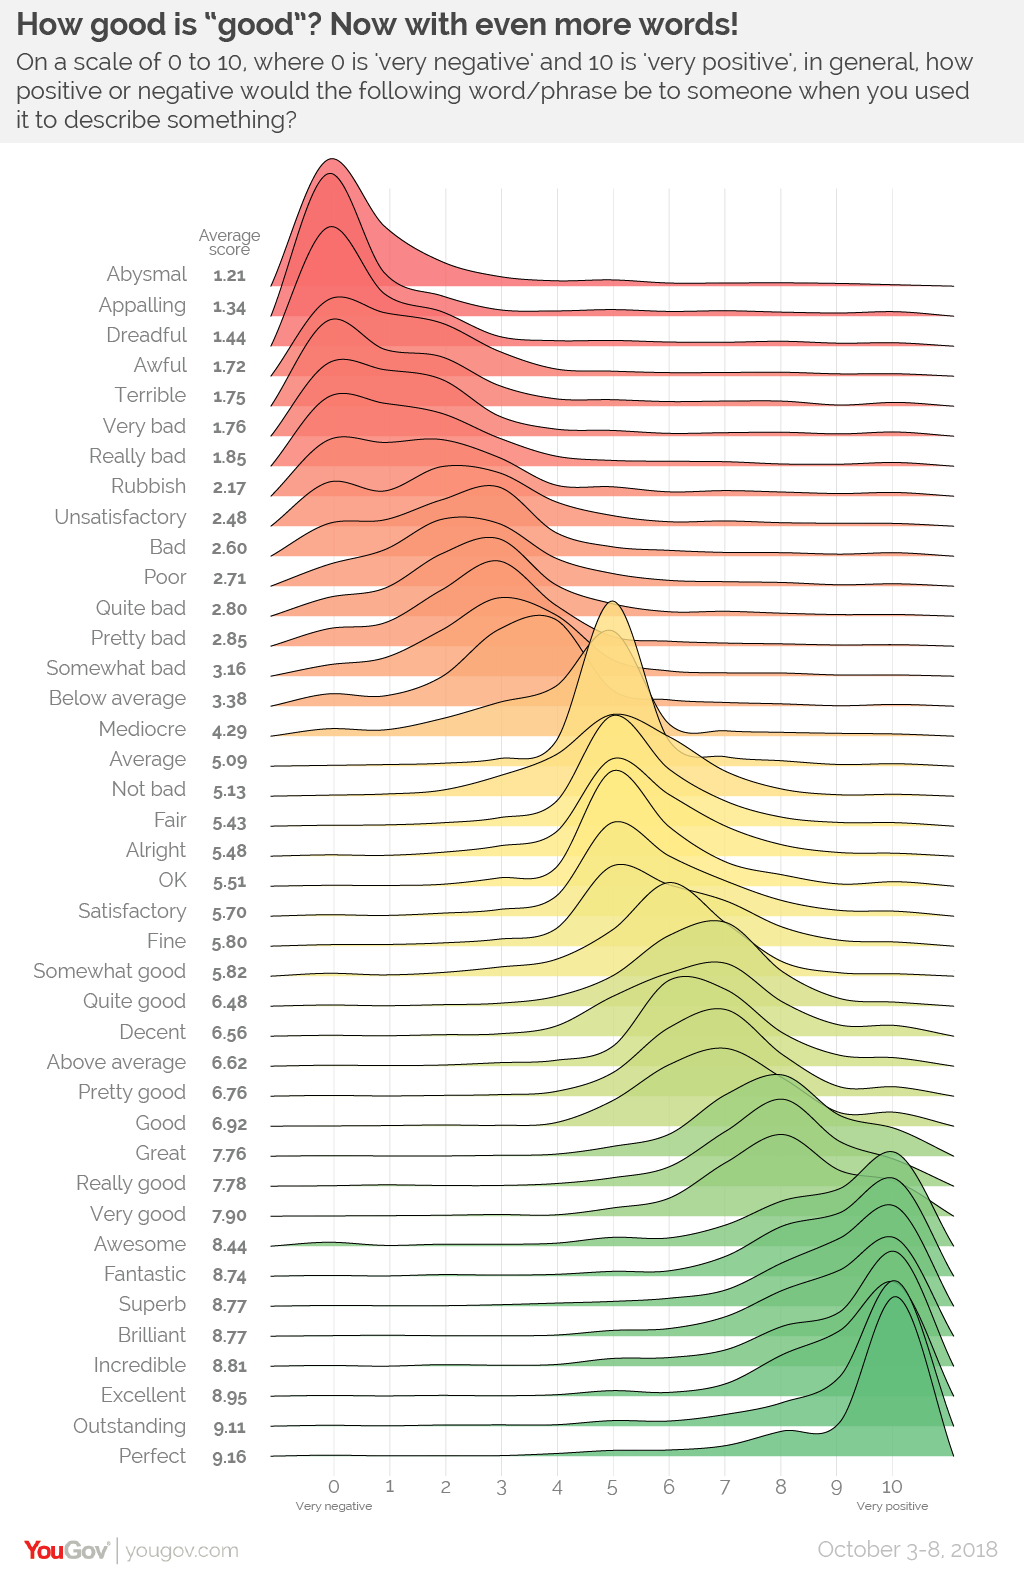
\includegraphics[height=.8\textheight]{../figures/howgood.png}
  \caption{\emph{How good is \foreignquote{english}{good}?} Figure
    réalisée à l'aide d'un lissage par noyau, à partir d'un sondage
    effectué au près d'au moins 1005 citoyens britanniques
    (l'échantillon varie pour chaque adjectif). Extrait de
    \textcite{Smith2018}}
  \label{fig:how_good}
\end{figure}

Dans la littérature, le terme imprécis est régulièrement utilisé comme
synonyme de vague, notamment par \textcite{Zadeh1965} et dans une
grande partie des travaux se rattachant à la logique floue. Par
métonymie, le terme flou\footnote{} est également employé dans le sens
de vague, imprécis. C’est, par exemple, le cas lorsque
\textcite{Lagacherie1996} parlent de \enquote{\emph{fuzziness}} ou
encore quand \textcite[p. 218]{Brunet1992} définissent le \emph{flou}
comme : \enquote{la partie d’un système ou d’un espace dont les
  contours et les limites sont, soit imparfaitement connus ou
  connaissables, soit instables, soit imprécis \textelp{}}. De
nombreux autres termes sont ponctuellement utilisés, rendant la
terminologie confuse (\autoref{tab:termes_vague}). Pour rendre notre
propos le plus clair possible, nous n’emploierons le terme flou que
pour qualifier des formalisations fondées sur la théorie des
sous-ensembles flous de \textcite{Zadeh1965}. De plus, pour rester le
plus proche possible du vocabulaire utilisé en géomatique nous
préférerons le terme imprécis à celui de vague.

\begin{table}
  \centering
  \begin{tabular}{rL{6cm}L{6cm}}
  \toprule
  & {\bfseries Anglophone} & {\bfseries Francophone} \\
  \midrule
   {\bfseries Précis} & \emph{Crisp, Sharp, Well defined, Fiat boundaries} & Net
  \\
  {\bfseries Imprécis} & \emph{Fuzzy, Indeterminate, Undefined, Uncertain,
                         Ill-Defined, Unclear, Vagueness, Bona fide boundaries} & Flou, Incertain, Vague
  \\
  \bottomrule
\end{tabular}
  \caption{Termes utilisés dans la littérature comme synonymes de
    précis et d’imprécis}
  \label{tab:termes_vague}
\end{table}

La notion d’\emph{imprécision} peut être associée à d’autres concepts,
comme l’\emph{exactitude} chez \textcite{Russell1923}, que l’on
retrouve chez \textcite{Bouchon-Meunier1995, Bouchon-Meunier2007} sous
le nom d’\emph{incertitude}. Ici, l’\emph{incertitude} est entendue
comme le doute que l’on peut avoir sur la validité d’une connaissance
\autocite{Bouchon-Meunier1995}. L’\emph{imprécision} et
l’\emph{incertitude} sont foncièrement liées et varient généralement
en sens inverse \autocite{Russell1923}. Ainsi, si la proposition :
%
\begin{enumerate*}[label=(\alph*)]
\item \enquote{la distance de la Terre à la Lune est de
    \SI{384397}{\kilo\meter}} est plus \emph{précise} que la
  proposition : \label{p1}
\item \enquote{la distance de la Terre à la Lune est d’environ
\SI{384000}{\kilo\meter}}, \label{p2}
\end{enumerate*}
%
mais la seconde proposition est plus \textsf{certaine} car, son cadre
de validité (la plage de valeurs de la distance Terre-Lune) est plus
large. On peut en effet, considérer que la proposition \ref{p2} reste
vraie pour une distance réelle de \num{383500} ou
\SI{384999}{\kilo\meter} alors que la moindre variation de l’ordre
d’un kilomètre suffit à invalider la première proposition
\ref{p1}. Dans certains cas, et notamment lorsque ces notions sont
appliquées à des objets spatiaux, il peut être délicat de distinguer
ces deux concepts. Cependant, ils sont fondamentalement différents :
l’\emph{imprécision} est une caractéristique invariable, alors que
l’\emph{incertitude} est contextuelle. Pour reprendre l’exemple
précédent, la proposition \ref{p2} est imprécise et le restera quel
que soit le contexte, alors que sa certitude dépend des connaissances
de l’observateur. La véracité des propositions \ref{p1} et \ref{p2}
est, toutes choses égales par ailleurs, invariable, mais la certitude
de cette véracité est contextuelle.

L’\emph{imprécision} et l’\emph{incertitude} sont également associées
à la notion d’\emph{incomplétude}, qui désigne une connaissance
partielle. Ceci est dû au fait qu’un manque de connaissances peut
entraîner des \emph{incertitudes}, mais également des
\emph{imprécisions}
\autocite{Bouchon-Meunier1995,Bouchon-Meunier2007}. Pour
\textcite{Bouchon-Meunier1995} et plus généralement pour la communauté
de chercheurs en intelligence artificielle, la composition de ces
trois concepts définit la notion d’\emph{imperfection.} Dans la suite
de ce document, nous travaillerons à partir de cette typologie, même
si de nombreuses autres typologies de concepts ont cependant été
proposées, que ce soit dans le domaine de l’intelligence artificielle
ou de la géomatique \autoref{Fisher2006}.

\subsubsection{Imprécision et géographie}

Les objets et les concepts géographiques n’échappent évidemment pas à
l’imprécision. Ainsi, \textcite{Russell1923} mentionnait déjà
l’existence d’objets dont la délimitation spatiale est imprécise, tel
que le système solaire. De nombreux autres objets spatiaux imprécis
ont été identifiés, comme l’illustre l’exercice de définition du
\emph{Brownfield} \footnote{}, entrepris par \textcite{Alker2000} et
relevé par \textcite{Bennett2001}, qui y voit un bon exemple de la
difficulté d’identifier une délimitation satisfaisante d’espaces
naturels. Le B\emph{rownfield,} tout comme les forêts
\autocite{Bennett2001,Dilo2006,Fisher2006}, les montagnes
\autocite{Varzi2001,Varzi2015,Fisher2006,Chaudhry2008}, les vallées
\autocite{Schneider2003} ou même le Soleil \autocite{Simons1999},
appartiennent à cette catégorie d’objets spatiaux dont on ne peut
fixer une limite. Cette énumération pourrait laisser penser que
l’imprécision ne concerne pas les artefacts, pourtant l’expérience de
\textcite{Perec1974} nuance cette affirmation. Comme l’indique
\textcite{Campari1996}, l’identification des frontières d’un artefact,
n’est pas aisée puisque dépendante du contexte d’observation. Ainsi,
la limite d’une ville ou d’un village est tout aussi vague que celle
d’une zone frontalière \autocite{Varzi2001, Fisher2006}, comme
l’illustre la grande variabilité des définitions du concept de ville.
Tous ces objets géographiques, généralement qualifiés de \emph{vagues}
\autocite{Erwig1997}, \emph{imprécis} \autocite{Winter2000},
\emph{flous} \autocite{Lagacherie1996} ou d’objets aux
\emph{frontières indéterminées} \autocite{Burrough1996}, s’opposent
aux objets dits \emph{nets} \autocite{Schneider2001} ou
\emph{précis}. \textcite{Smith1995, Smith1997, Smith2000} font usage
d’un vocabulaire très différent en opposant les \emph{fiat boundaries}
(\ie les frontières précises) qu’ils estiment profondément liées à un
processus cognitif, \emph{aux bona fide boundaries} caractérisant les
objets spatiaux dont la délimitation est univoque
\autocite{Varzi2015}. Pour \textcite{Couclelis1996}, les objets
géographiques nets sont d’avantage l’exception que la norme. Ce
constat est corollaire de l’avis
d’\textcite[p. 200]{OddAmbrosetti1987}, pour qui \enquote{\textelp{}
  il est problématique et généralement arbitraire de tracer des
  limites \textelp{}}\footnote{}, limites qui, selon
\textcite[P. 106]{Brunet2001}, sont \enquote{\textelp{} indécises,
  fuyant sans cesse devant l’analyse, et même, localement
  indécidables}. \textcite{Dutozia2014} considèrent, quant à eux, que
\enquote{\textelp{} l’espace géographique est par essence flou
  \textelp{}}.

Ainsi, si les concepts présentés jusqu’ici nous semblent actuellement
peu utilisés en géographie, de nombreuses notions et objets entrant
dans le champ d’étude de la discipline y sont fondamentalement
liés. C’est notamment le cas des différents maillages administratifs,
comme les régions \autocite{Brennetot2014}, mais également les
frontières \autocite{Brunet1992}, les seuils
\autocite{Brunet1992,Levy2013}, les discontinuités
\autocite{Brunet1992,Brunet1997}, les franges \autocite{Brunet1992},
les confins \autocite{Brunet1997} ou encore les fronts pionniers
\autocite{Brunet1992}, qui, comme tous les concepts dérivant de la
notion de \emph{limite} sont généralement définis comme pouvant être
graduels ou progressifs \autocite{Brunet1992,Levy2013}, c’est-à-dire
foncièrement \emph{imprécis.} La question de la formalisation des
objets spatiaux imprécis a cependant été abordée en géographie, avant
même le développement des systèmes d’information géographiques
\autocite{Robinson2003}. Dans les années 1970 où, à la suite de
l’élaboration de la théorie des sous-ensembles flous
\autocite{Zadeh1965}, plusieurs géographes, rattachés au courant
\emph{béhavioriste}, tels que \textcite{Gale1972,Gale1976},
\textcite{Pipkin1978} ou \textcite{Leung1979, Leung1987} ont identifié
les problèmes que l’existence d’objets géographiques aux limites
imprécises pouvaient poser à la géographie. Parmi ces problèmes,
\textcite{Gale1976} a identifié la question de la
régionalisation. Cette problématique sera également abordée par
\textcite{Rolland-May1996,Rolland-May1999} lors de ses travaux sur la
définition de territoires de cohérence. Les travaux béhavioristes
aboutiront à la formalisation du concept d’objet géographique imprécis
à l’aide de la théorie des sous-ensembles flous
\autocite{Leung1987}. Ces travaux n’auront, semble-t-il, pas suffi à
inscrire durablement le concept d’imprécision dans le champ de la
géographie; puisque des publications ré-introduisant ce concept en
géographie, apparaîtront régulièrement. C’est notamment le cas de
\textcite{Fisher1998}, \textcite{Collins2000}, qui se fonderont
indépendamment sur l’exemple de la définition d’une montagne pour
introduire cette notion.

Parallèlement, \textcite{Rolland-May1984,Rolland-May1987} se fondera
notamment sur les travaux de \textcite{Gale1972,Gale1976} et
\textcite{Leung1979} pour développer le concept\emph{ d’espace
  géographique flou.} Cette dénomination qualifie la formalisation, à
l’aide de la théorie des sous-ensembles flous, de l’espace tel que
conceptualisé en géographie. Ce travail permettra à Rolland-May de
proposer une définition formelle de notions courantes utilisées en
géographie, telles que les franges \autocite{Rolland-May1987},
définies comme la limite floue d’un espace géographique, ou les
discontinuités, décrites comme une configuration particulière
d’ensemble flou \autocite{Rolland-May2003}. Les différents travaux de
\bsc{Rolland-May} autour de la question de l’imprécision en géographie
ont permit à différents chercheurs d’aborder différemment des
questions géographiques \textcite{Dutozia2014}, comme, par exemple, de
\textcite{Ruffray2004}, qui feront usage des concepts développés par
\bsc{Rolland-May} pour quantifier la cohérence de territoires, ou
\textcite{Didelon2011} qui emploient la logique floue pour exploiter
des cartes mentales.

\subsubsection{L’imprécision spatiale}

Nous proposons d’utiliser le terme d’imprécision spatiale pour décrire
l’application du concept d’imprécision aux objets spatiaux. Par ce
terme, nous entendons qualifier toutes les situations où un objet
spatial, quelle que soit sa nature, voit ses limites difficilement
identifiables. Il s’agit donc d’un concept ne portant que sur la
dimension spatiale et non sur les autres aspects. Par exemple, la
difficulté de délimitation spatiale d’un objet géographique tel que la
forêt entre dans le cadre de l’imprécision spatiale. Ce n’est
cependant pas le cas de la difficulté de définition du concept en
lui-même, il s’agit dans ce cas d’imprécision sémantique. Ainsi,
l’imprécision spatiale n’est qu’un cas spécifique du concept général
d’imprécision, précédemment présenté, mais son cadre d’application et
les spécificités de la question spatiale justifient la définition d’un
nouveau concept.  Pour illustrer ce concept, nous allons nous appuyer
l’exemple de la définition des rives d’un lac artificiel. La
\autoref{fig:lim_champ} est une orthophotographie de la partie ouest
du lac du Chambon (Isère) sur laquelle a été dessinée la limite de
l’eau. On peut cependant se demander si la limite que nous avons
tracée est une délimitation satisfaisante de l’objet lac. En effet, le
niveau de l’eau est amené à bouger au cours du
temps. L’orthophotographie permet d’identifier ces zones, dépourvues
de végétation et situées au-delà de la limite représentée sur la
\autoref{fig:lim_champ}. On peut donc tracer une seconde limite, celle
de la zone atteignable par les eaux (\autoref{fig:lim_champ_alt}) et
considérer que c’est ce nouveau tracé qui délimite l’objet lac.

\begin{figure}
  \centering
  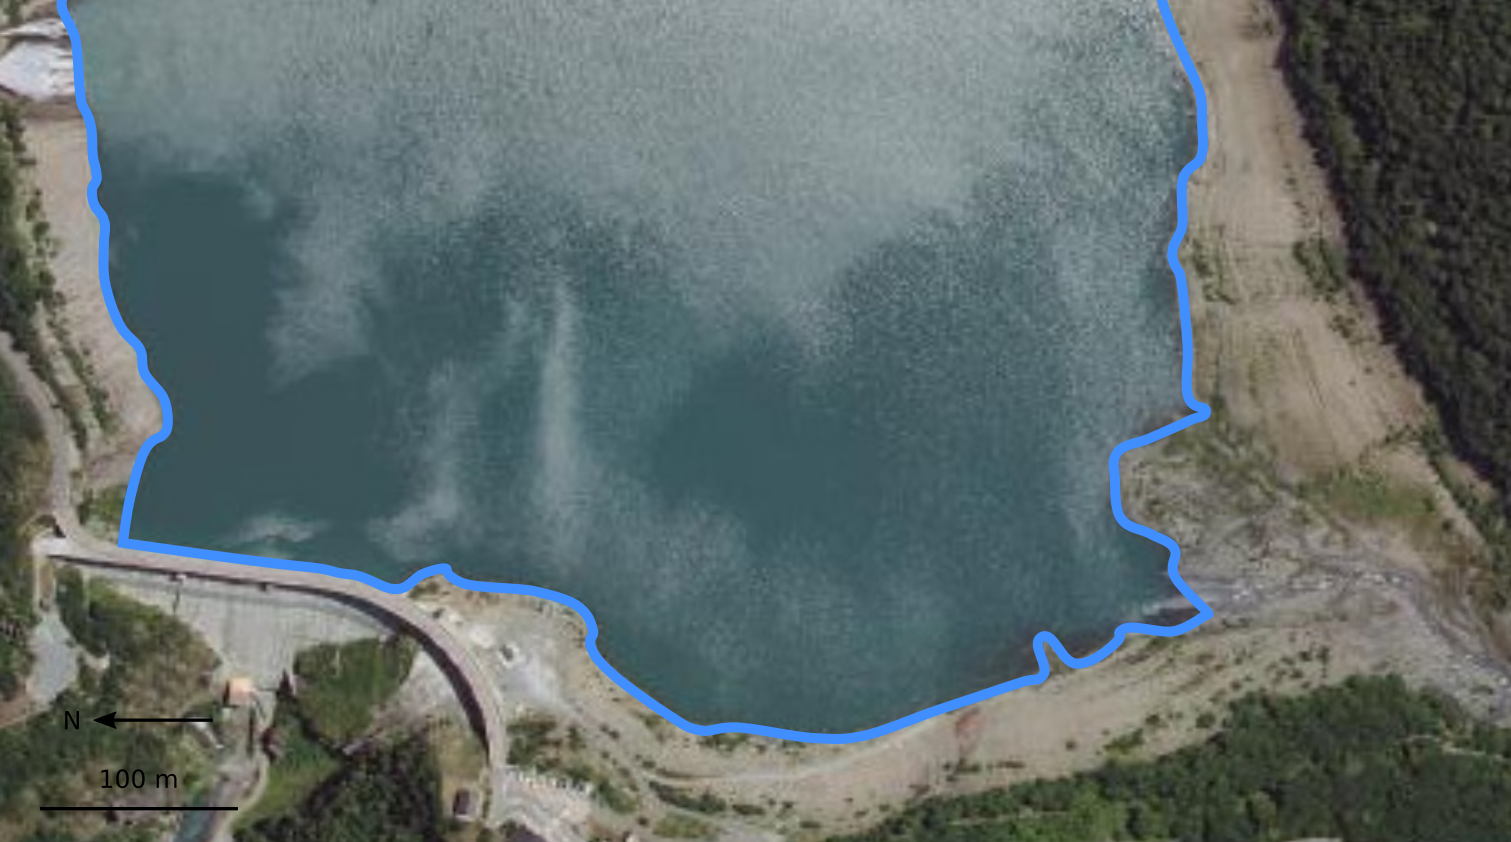
\includegraphics{../figures/fig1.png}
  \caption{Saisie manuelle de la limite du lac du Chambon. Extrait de
    \textcite{Bunel2020}.}
  \label{fig:lim_champ}
\end{figure}

\begin{figure}
  \centering
  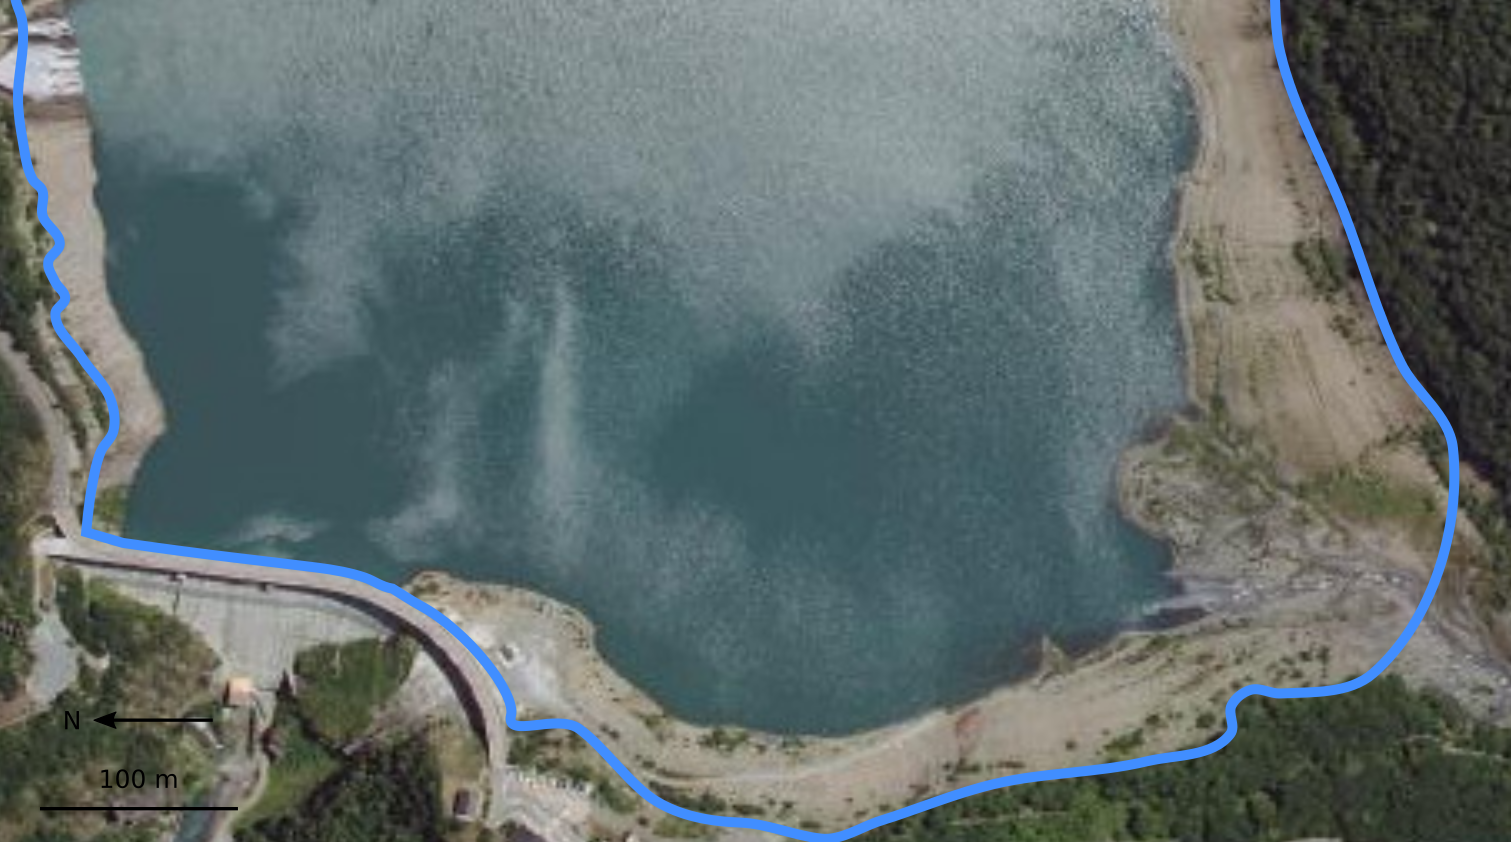
\includegraphics{../figures/fig2.png}
  \caption{Saisie manuelle d'une limite alternative. Extrait de
    \textcite{Bunel2020}.}
  \label{fig:lim_champ_alt}
\end{figure}

Toutefois, aucune de ces délimitations n’est réellement
satisfaisante. Peut-on considérer qu’une zone pouvant être découverte
appartient autant à l’objet \enquote{lac} qu’une zone qui est toujours
recouverte d’eau ? À l’inverse, peut-on considérer qu’une zone
intermittemment située sous l’eau n’appartient pas au lac de la même
manière que la forêt située à plusieurs dizaines de mètres de là ?
Cette difficulté de délimitation est liée, comme nous l’expliquions
précédemment, à \emph{l’imprécision} de l’objet \enquote{lac.} On ne
peut en définir une limite précise autrement qu’arbitrairement. Nous
avons cependant pu tracer deux limites \emph{précises}\footnote{},
celle de la zone recouverte d’eau (\autoref{fig:lim_champ}) et celle
de l’étendue maximale du lac (\autoref{fig:lim_champ_alt}). Ces deux
frontières délimitent une aire de transition, entre le lac et son
extérieur (\autoref{fig:lim_champ_imp}), c’est-à-dire la frontière du
lac.

\begin{figure}
  \centering
  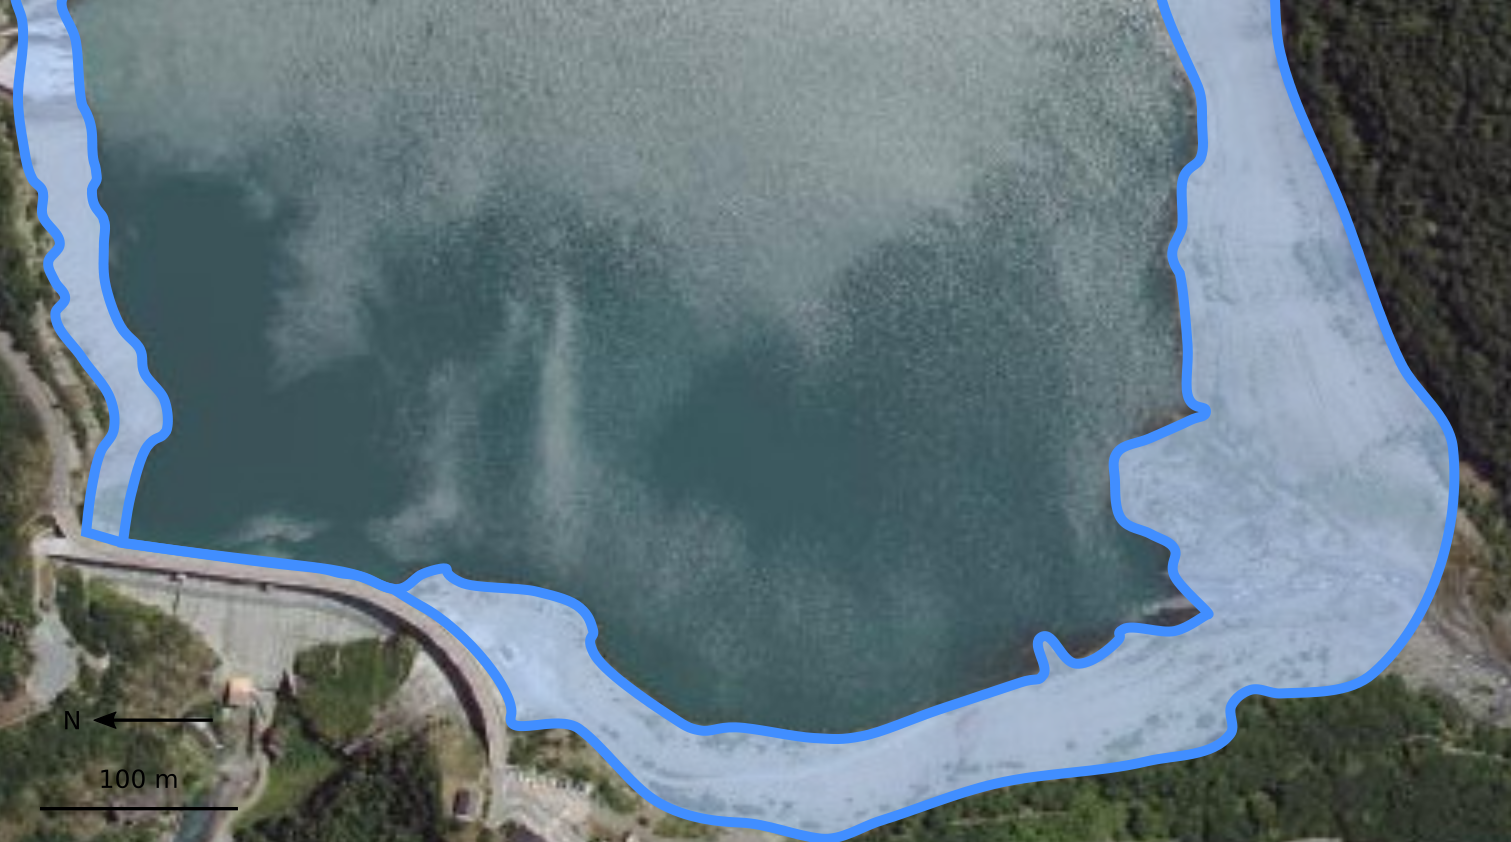
\includegraphics{../figures/fig3.png}
  \caption{Mise en évidence de la limite imprécise du lac. Extrait de
    \textcite{Bunel2020}.}
  \label{fig:lim_champ_imp}
\end{figure}

De même que pour l’imprécision, le concept d’incertitude ne voit pas
sa définition générale impactée par la prise en compte de la dimension
spatiale. Cependant, la multiplicité des termes utilisés dans la
littérature, les contradictions entre auteurs et les représentations
graphiques utilisées pour présenter les concepts sont sources de
nombreuses confusions entre les concepts d’imprécision et
d’incertitude spatiale.

Comme expliqué précédemment, l’incertitude qualifie le doute que l’on
peut avoir sur une connaissance. On peut donc définir l’incertitude
spatiale comme le doute sur la position d’un objet. Ce concept peut
être, tout du moins selon \textcite{Tossebro2002}, décomposé en deux
éléments : l’\emph{incertitude positionnelle} et l’\emph{incertitude
  morphologique.} \emph{L’incertitude positionnelle} qualifie un doute
sur la position d’un objet spatial. \textcite{Tossebro2008} prennent
comme exemple l’estimation par sonar de la position d’un
sous-marin. Ce cas offre une bonne opportunité pour distinguer
\emph{imprécision} et \emph{incertitude spatiale.} L’objet sous-marin,
est, de part sa nature d’artefact, net ; l’identification de ses
frontières, à une échelle donnée, ne pose pas de problèmes. Cependant,
sa position est mal connue, puisqu’estimée à l’aide d’un outil peu
précis qui ne peut qu’estimer une zone de présence. La position de
l’objet est donc \emph{incertaine.} \emph{L’incertitude morphologique}
qualifie, quant à elle, un doute sur la forme de l’objet,
c’est-à-dire. sur la position de sa frontière. C’est pourquoi on peut
considérer que \emph{l’incertitude morphologique} correspond à une
\emph{incertitude positionnelle} portant uniquement sur la frontière
de l’objet. On peut prendre comme exemple une nappe phréatique, dont
l’étendue ne peut être qu’estimée par des relevés terrain. Il est donc
possible de savoir si la nappe est présente ou non en un point de
mesure, mais non d’en définir la frontière, ce qui se traduit par une
\emph{incertitude} sur la position de la frontière, \ie une
\emph{incertitude morphologique} telle que déqfinie par
\textcite{Tossebro2002,Tossebro2008}. La proximité des concepts
\emph{d’incertitude morphologique} et \emph{positionnelle} peut
expliquer pourquoi les autres définitions de l’\emph{incertitude}
spatiale, notamment issues des travaux de \textcite{Clementini2008},
\textcite{Lagacherie1996}, \textcite{Freksa1996}\footnote{} ou
\textcite{Schneider1999} fusionnent ces deux
notions. \textcite{Dutton1992}, quant à lui, inclut ces deux notions
dans sa définition de \emph{l’incertitude positionnelle.}

On peut illustrer la notion \emph{d’incertitude spatiale} en
réutilisant l’exemple de la délimitation du lac du Chambon (Figures
\ref{fig:lim_champ} et \ref{fig:lim_champ_alt}). Lorsque nous avons
tracé la limite du niveau maximal de l’eau
(\autoref{fig:lim_champ_alt}), nous nous sommes appuyés sur
  l’emplacement de la végétation. Cependant, dans certains cas,
  notamment pour la rive sud du lac, il s’est avéré difficile
  d’identifier la bonne limite et ce à cause de la présence de
  certaines poches de végétation. Ainsi, la frontière sud de l’étendue
  maximale du lac est \emph{incertaine}, son tracé est contestable,
  mais uniquement à cause de notre manque de connaissances. Il ne
  s’agit pas d’\emph{imprécision}. La \autoref{fig:lim_champ_inc}
  représente une zone au sein de laquelle le tracé exact de la
  frontière est \emph{incertain}, c’est-à-dire qu’au sein de cette
  zone, tous les tracés sont envisageables\footnote{}. Ainsi, le lac
  du Chambon, rentre dans la catégorie des objets spatiaux à la fois
  \emph{imprécis} et \emph{incertains}.

\begin{figure}
  \centering
  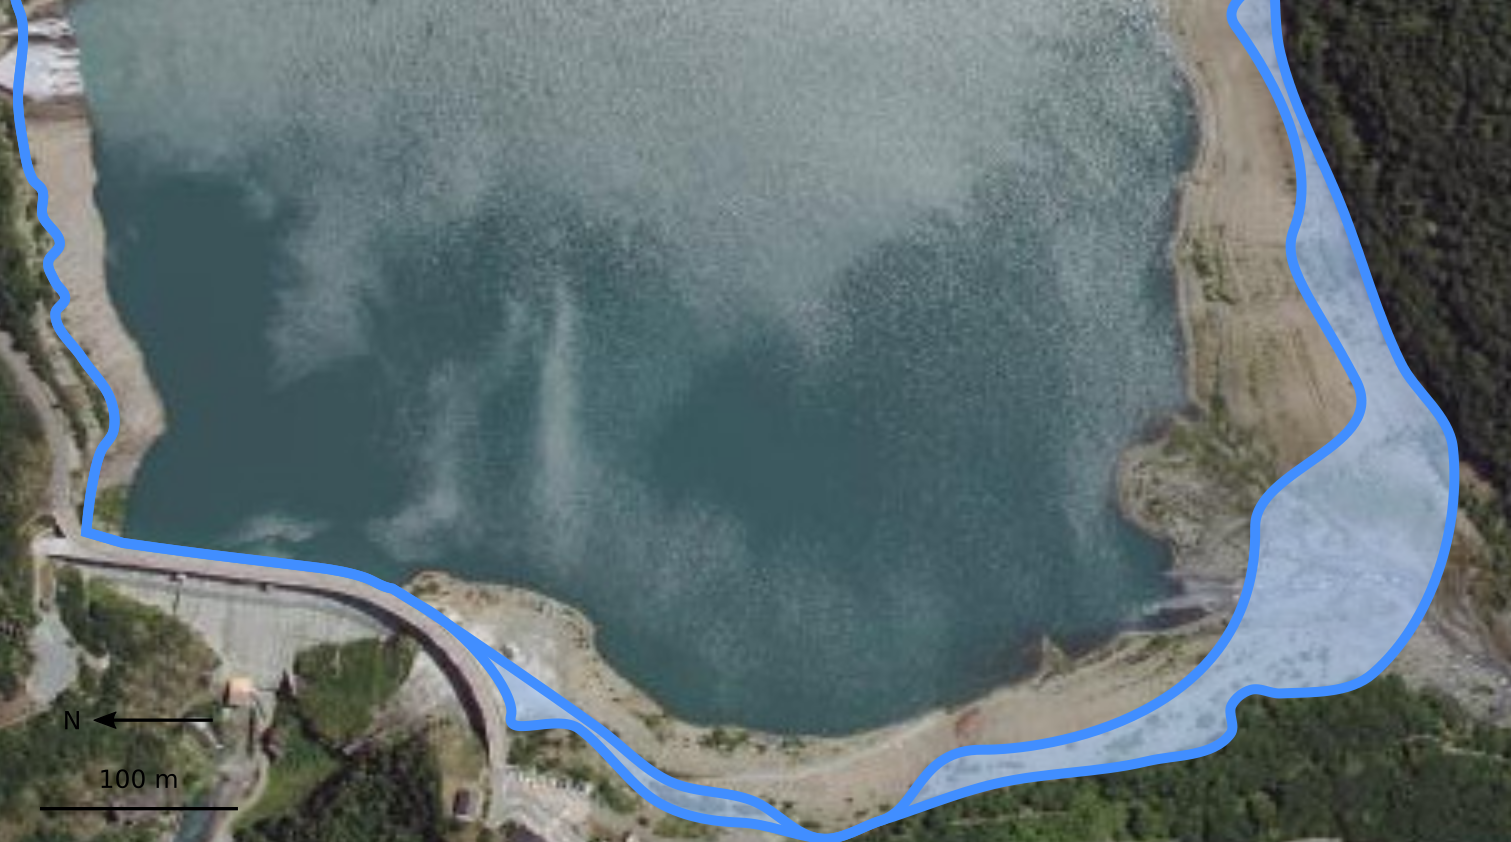
\includegraphics{../figures/fig4.png}
  \caption{Mise en évidence de l'incertitude pour la limite des hautes
    eaux. Extrait de \textcite{Bunel2020}.}
  \label{fig:lim_champ_inc}
\end{figure}

\emph{L’incertitude} et \emph{l’imprécision spatiales} peuvent
cohabiter, comme dans le cas du lac du Chambon. La figure
\ref{fig:inc_vs_imp} donne un aperçu plus théorique de la différence
qu’il peut y avoir entre ces deux notions. \emph{L’incertitude
  spatiale} est représentée par plusieurs frontières, illustrant le
doute sur la position de la limite de l’objet. \emph{L’imprécision
  spatiale} est, quant à elle, représentée par une bande, marque d’une
frontière progressive, non réductible à une ligne.

\begin{figure}
  \centering
  \begin{tabular}{rC{5cm}C{5cm}}
  \toprule
  & \textbf{Précis} & \textbf{Imprécis} \\
  \midrule
  \textbf{Certain} &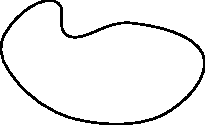
\includegraphics{../figures/incVSimpP1.pdf} & 
\includegraphics{../figures/incVSimpP2.pdf}\\
  \textbf{Incertain} &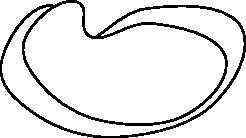
\includegraphics{../figures/incVSimpP3.pdf} & 
\includegraphics{../figures/incVSimpP4.pdf}\\
  \bottomrule
\end{tabular}

  \caption{Distinction entre les notions d’imprécision et
    d'incertitude spatiale (pour des raisons de lisibilité seule la
    frontière de l’objet spatial est représentée). D'après
    \textcite{Bunel2020}.}
  \label{fig:inc_vs_imp}
\end{figure}

De façon similaire à ce qui a été décrit précédemment,
\emph{l’incertitude et l’imprécision spatiales} sont liées. Par
exemple, le fait qu’un objet géographique soit \emph{imprécis}
complexifie l’identification de sa frontière, ce qui se traduit par
une \emph{incertitude morphologique} \autocite{Lagacherie1996}. De
plus, la \emph{précision} et la \emph{certitude} des attributs d’un
objet géographique sont fortement liées à la \emph{précision} et à la
\emph{certitude spatiale} de ce même objet et inversement
\autocite{Mark1989}. Ainsi, la définition d’un objet géographique à
partir de données imprécises le sera elle-même, et le recueil
d’informations au sein d’un objet géographique dont la frontière est
\emph{incertaine} ne pourra qu’être une opération qui l’est tout
autant.

Différents auteurs ont listé des facteurs expliquant l’apparition de
\emph{l’imprécision} et de \emph{l’incertitude spatiales}, comme
\textcite{Freksa1996,Dutton1992} qui identifient quelques facteurs
explicatifs. D’autres travaux \autocite{Hadzilacos1996,Evans2008} vont
plus loin en proposant une typologie plus poussée de ces différents
facteurs. Enfin, des typologies d’objets spatiaux \emph{imprécis,}
comme celle proposée par \textcite{Liu2019}, permettent d’identifier
d’autres causes, inhérentes au processus de construction des objets
spatiaux.

Une première cause de \emph{l’imprécision spatiale,} correspondant à
la majorité des exemples précédents, est liée à \emph{l’imprécision
}de la définition. Par exemple, l’objet géographique
\enquote{montagne}, n’est pas (seulement) \emph{imprécis} à cause
d’une quelconque difficulté technique limitant la précision des
mesures, il l’est car le concept montagne n’est pas suffisamment clair
pour permettre la délimitation précise d’une portion d’espace. C’est
généralement \emph{l’imprécision du concept} qui rend \emph{l’objet
  géographique imprécis} \autocite{Freksa1996}. \emph{L’imprécision du
  concept} est à distinguer des \emph{définitions concurrentes,} ce
qu’\textcite{Evans2008} nomment
\foreignquote{english}{\emph{definitional disagreement}}. C’est, par
exemple, le cas des frontières contestées, nécessairement mutuellement
exclusives, qui, même si définies aussi précisément que possible, ne
permettent pas de construire une frontière unique, sinon en admettant
une part d’incertitude spatiale. Par conséquent, le
\foreignquote{english}{\emph{definitional disagreement}}, et plus
généralement, l’existence de géométries concurrentes pour un même
individu \autocite{Hadzilacos1996}, sont une source
\emph{d’incertitude,} inhérente au choix d’une possibilité parmi
l’ensemble des possibles.

Cependant, l’imprécision d’une définition peut être souhaitée.
\textcite{Hadzilacos1996} parle alors de
\foreignquote{english}{\emph{don't care \textins{boundaries}}}. C’est,
par exemple, un cas que l’on retrouve fréquemment lors de la
description en langage naturel d’une position. Un exemple de
\textcite{Bateman2010}, illustre bien cette situation, si pour décrire
sa position, une personne dit : \enquote{Je suis à la Poste}, on ne
peut pas en conclure qu’elle est située à l’intérieur d’une agence
postale. En effet, si la file d’attente sort du bâtiment, cette
description sera toujours valable. La limite de \enquote{la Poste} est
donc peu précise, mais dans ce contexte, il n’est pas nécessaire
qu’elle le soit davantage. L’information que le locuteur cherche à
communiquer est sa proximité et son interaction avec une agence
postale, et non sa présence au sein du bâtiment.

La dimension temporelle peut également être une source
d’imprécision. \textcite{Hadzilacos1996,Liu2019} mentionnent
respectivement l’existence de \enquote{time-varying
  \textins{boundaries}} et de \enquote{Dynamic boundary objects} pour
qualifier des objets géographiques dont la frontière varie dans le
temps. C’est, par exemple, le cas d’un front de mer. Pour ce type
d’objets, définir une frontière nécessite de \enquote{synthétiser} les
différentes évolutions temporelles, ce qui conduit nécessairement à
une frontière \emph{imprécise}. Dans ce cas \emph{l’imprécision
  spatiale} est un artefact, né de la modélisation atemporelle d’un
objet qui ne l’est pas.

On peut également relever des aspects plus techniques, comme
l’imprécision liée aux instruments de mesure ou au producteur de
données \autocite{Follin2019} et plus généralement au processus de
production de données
\autocite{Dutton1992,Evans2008,Follin2019}. D’autres points plus
spécifiques peuvent également être identifiés, comme les limites des
modèles de représentation des données
\autocite{Dutton1992,Follin2019}. Il est par exemple impossible de
représenter tous les nombres réels informatiquement à cause de la
précision finie des nombres flottants utilisés pour les figurer.

Enfin, il convient de noter que \emph{l’imprécision} et
\emph{l’incertitude} peuvent \enquote{se transmettre} lors de la
définition de nouveaux objets à partir de mesures
\autocite{Dutton1992} ou d’objets géographiques imprécis
\autocite{Liu2019,Follin2019}. On peut, dans ce cas, parler
\emph{d’imprécision \emph{et} d’incertitude de second ordre.} C’est ce
phénomène que décrivent \textcite{Liu2019} lorsqu’ils définissent les
\enquote{element-clustering objects}, des objets spatiaux imprécis
construits par l’agrégation d’autres objets (flous ou nets), et les
\enquote{object-referenced objects}, construits par subdivision
d’objets spatiaux imprécis.

\subsection{La modélisation de l'imprécision spatiale}

La question de la modélisation de l’imprécision a conduit au
développement de plusieurs théories mathématiques, dont la plus connue
est la théorie des sous-ensembles flous \autocite{Zadeh1965}. Nous
avons choisi de nous centrer sur la présentation de cette théorie, car
nous n’avons pas identifié dans la littérature des utilisations de
théories alternatives comme la théorie des fonctions de
croyances. Quant aux travaux basés sur la théorie des probabilités
\autocite{Tossebro2002,Tossebro2008}, ceux-ci traitent de la
modélisation de l’\emph{incertitude}, c’est pourquoi nous ne les
incluons pas dans cet article.

% \subsubsection{La théorie des fonctions de croyance}

% La \emph{théorie des fonctions de croyances} (également nommée
% \emph{théorie de l'évidence} ou \emph{théorie de
%   \bsc{Dempster-Shafer}}) a été proposée par \textcite{Shafer1976} à
% la suite des travaux de \textcite{Dempster1967}.

% Dans la théorie des fonctions de croyances on s'intéresse à un certain
% nombre d'hypothèses \(H_i\) dont l'ensemble forme le cadre de
% discernement \(\Theta\). L'ensemble de tous les sous-ensembles de
% \(\Theta\) correspond au référentiel de définition, noté
% \(2^\Theta\). Ce dernier représente tous les couples d’hypothèses
% possibles.

% La théorie des fonctions de croyance permet d'attribuer une telle fonction

\subsubsection{La théorie des sous-ensembles flous}

La théorie des sous-ensembles flous, ou, par abus de langage, théorie
des ensembles flous \autocite{Bouchon-Meunier2007}, proposée par
\textcite{Zadeh1965}, vise à proposer un cadre théorique permettant de
modéliser des appartenances partielles à une classe
d’objets. \textcite{Bouchon-Meunier1995} présente les sous-ensembles
flous comme un \enquote{assouplissement} des ensembles
\enquote{classiques}, ici qualifiés de \enquote{nets} \footnote{}
\autocite{Smithson2006}. La possibilité de modéliser des appartenances
partielles permet à la théorie des sous-ensembles flous de modéliser
l’imprécision des connaissances, ce qui en fait un candidat idéal pour
la modélisation d’objets spatiaux imprécis.

Un ensemble flou $A$ est défini comme un couple composé d’un ensemble
net $X$ et d’une fonction $f_A$ nommée fonction d’appartenance :

\begin{equation}
  A = (X, f_A)  
\end{equation}

La fonction $f_A$, associe à chaque élément de X une valeur comprise
dans l’intervalle [0,1], nommée degré d’appartenance. Cette valeur
peut être interprétée comme une mesure de l’appartenance d’un élément
à $X$. Par exemple, si l’on définit $X$ comme l’ensemble des personnes
de grande taille, le degré d’appartenance qualifie l’appartenance
d’une personne à cet ensemble. Une personne mesurant 2,10 m aura un
degré d’appartenance de 1, i.e. qu’elle est considérée comme grande. À
l’inverse, une personne mesurant 1,75 m aura un degré d’appartenance
compris entre 0 et 1 (0,6 par exemple), traduisant une appartenance
partielle à l’ensemble des personnes de grande taille, ce qui revient
à dire qu’il s’agit d’une personne grande, mais pas totalement.

De la même manière, le degré d’appartenance peut illustrer
l’appartenance d’une position à un objet spatial. Par exemple, la
figure \ref{fig:champ_flou} illustre la représentation du lac du
Chambon à l’aide d’un sous-ensemble flou, les positions situées dans
la zone d’imprécision (\autoref{fig:lim_champ_imp}) se voient
attribuer un degré d’appartenance inférieur à 1. Ce degré devient nul
au-delà de la seconde frontière (\autoref{fig:lim_champ_alt}).

\begin{figure}
  \centering
  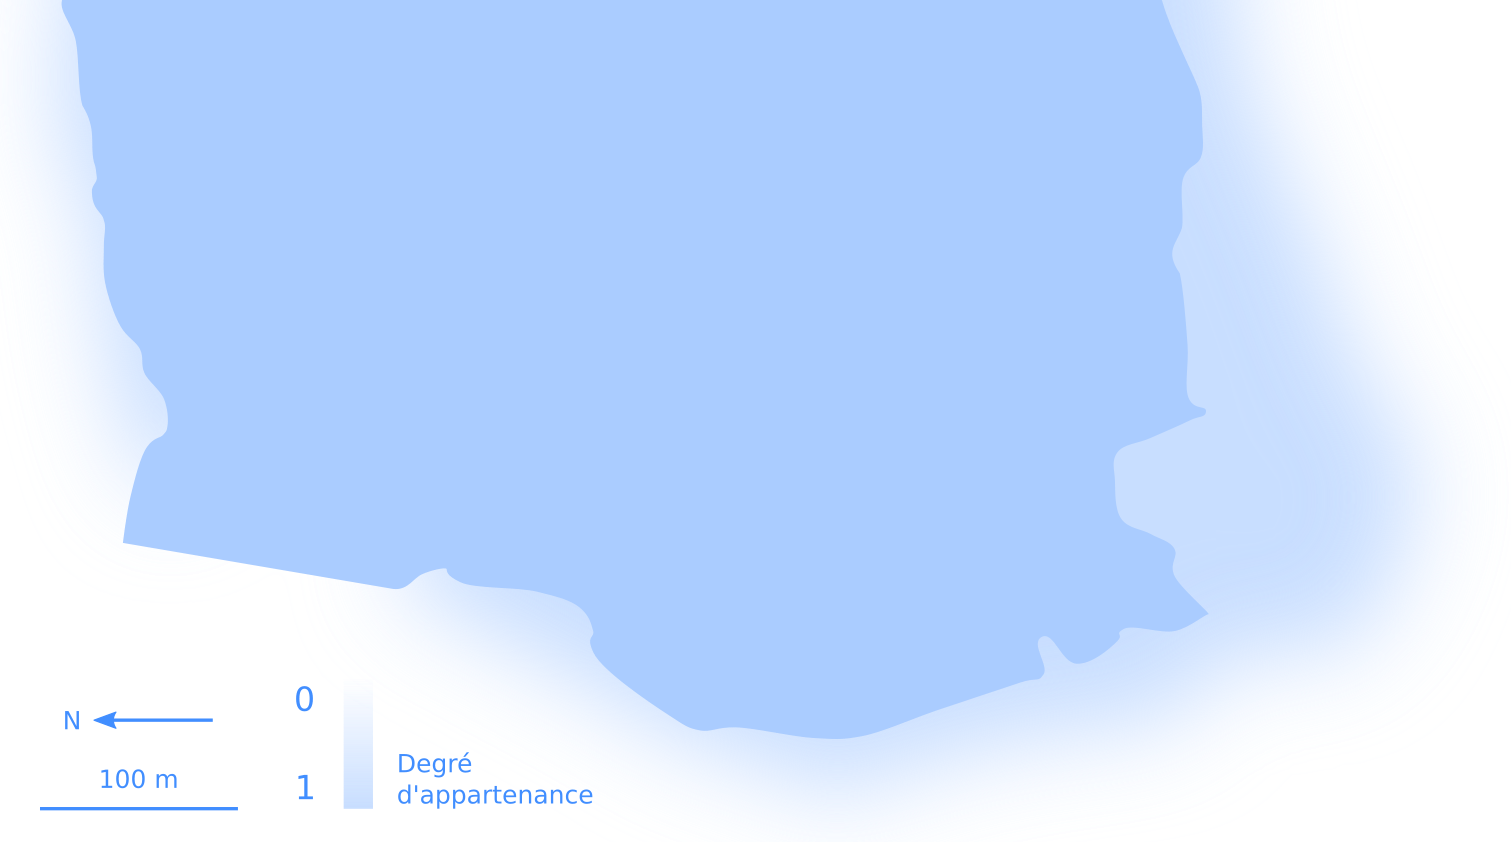
\includegraphics{../figures/fig6.png}
  \caption{Illustration de la modélisation du lac du Chambon à l’aide
    de la théorie des sous-ensembles flous. Extrait de
    \textcite{Bunel2020}.}
  \label{fig:champ_flou}
\end{figure}

L’ensemble des éléments ayant un degré d’appartenance non nul permet
de définir le support $S$ de l’ensemble :

\begin{equation}
  S(A) = \{x ∈ X \mid f_A(x) > 0\}
\end{equation}

Avec $X$ un ensemble net, $x$ un élément de l’ensemble $X$. Le noyau
$N$ de l’ensemble correspond, quant à lui, à l’ensemble des éléments
ayant un degré d’appartenance égal à 1 :

\begin{equation}
  N(A) = \{x ∈ X \mid f_A(x) = 1\}
\end{equation}

Si $A$ et $B$ sont deux sous-ensembles flous d’un même ensemble $X$,
$A$ et $B$ sont égaux, si et seulement si, pour tout élément de $X$,
le degré d’appartenance aux sous-ensembles $A$ et $B$ est égal, soit :

\begin{equation}
  A = B\ ssi\ ∀x ∈ X, f_A(x) = f_B(x)
\end{equation}

Un sous-ensemble flou $A$ de $X$ est inclus dans un sous-ensemble flou
$B$ de $X$ si et seulement si, pour tout élément $x$ appartenant à
$X$, le degré d’appartenance de $x$ à $A$ est inférieur ou égal à son
degré d’appartenance à $B$ :

\begin{equation}
  A ⊆ B\ ssi\ ∀x ∈ X, f_A(x) ≤ f_B(x)
\end{equation}

Le complément $A^c$ d’un sous-ensemble flou $A$ de $X$ a pour fonction
d’appartenance :

\begin{equation}
  ∀x ∈ X, f_{A^C}(x) = 1 − f_A(x)
\end{equation}

Ainsi, pour reprendre l’exemple précédent, on peut construire le
complément de l’ensemble des personnes de grande taille, l’ensemble
des personnes qui ne sont pas de grande taille. Une personne de 2,10 m
aura un degré d’appartenance nul à ce second ensemble, et une personne
de 1,75 m de 0,4.

Zadeh (1965) définit l’intersection de deux sous-ensembles flous $A$
et $B$ de $X$ comme le sous-ensemble flou $C$ de $X$ dont la fonction
d’appartenance est la suivante :

\begin{equation}
  \label{eq:norm_zadeh}
  ∀x ∈ X, f_C (x) = \min(f_A(x), f_B(x))
\end{equation}

De manière analogue, l’union de deux sous-ensembles flous $A$ et $B$
de $X$ est un sous-ensemble $C ∈ F(X)$ dont la fonction d’appartenance
est :

\begin{equation}
  \label{eq:conorm_zadeh}
  ∀x ∈ X, f_C (x) = \max(f_A(x), f_B(x))
\end{equation}

Par exemple, \emph{l’ensemble des personnes grandes et âgées} peut
être construit en intersectant \emph{l’ensemble des personnes âgées}
avec \emph{celui des personnes de grande taille.} En utilisant les
opérateurs proposés par \textcite{Zadeh1965}, une personne dont le
degré d’appartenance à ces deux ensembles est respectivement de 0,8 et
0,5, aura un degré d’appartenance à \emph{l’ensemble des personnes
  grandes et âgées} de 0,5. La \autoref{fig:zadeh_op} donne un aperçu
plus détaillé du comportement des opérateurs de \textcite{Zadeh1965}.

% Zadeh
\begin{figure}[hb]
  \begin{center}
    \subfloat[\emph{t-norme} de Zadeh (\autoref{eq:norm_zadeh})]{
      \begin{tikzpicture}
  \begin{axis}[
    width = 7cm,
    grid=none,
    view={-25}{30},
    xlabel=$x$,
    ylabel=$y$,
    zlabel=$\mu$]
    
    \addplot3 [surf, colormap/bone, domain = 0:1, samples = 20] {
      min(x,y) };
    
    \addplot3 [domain = 0:1, contour gnuplot = {number=11, labels={false}, draw color=black},
        samples=50,z filter/.code={\def\pgfmathresult{1}}]
        {min(x,y)};
  \end{axis}
\end{tikzpicture}
      \label{fig:zadeh_norm}
    }
    \subfloat[\emph{t-conorme} de Zadeh (\autoref{eq:conorm_zadeh})]{
      \begin{tikzpicture}
  \begin{axis}[
    width = 7cm,
    3d box,
    grid=major,
    tick align = outside,
    enlargelimits=false,
    line cap = round,
    clip = false,
    view={-25}{30},
    xtick={0,0.5,1},
    ytick={0,0.5,1},
    ztick={0,0.5,1},
    xlabel=$x$,
    ylabel=$y$,
    zlabel=$\mu$]
    \addplot3 [surf,  colormap/bone, domain = 0:1, samples = 20]
    { max(x,y) };
        \addplot3 [domain = 0:1, contour gnuplot = {number=11, labels={false}, draw color=black},
        samples=50,z filter/.code={\def\pgfmathresult{1}}]
        {max(x,y)};
  \end{axis}
\end{tikzpicture}
      \label{fig:zadeh_norm}
    }
    \caption{Opérateurs de Zadeh}
    \label{fig:zadeh_op}
  \end{center}
\end{figure}

Bien que les opérateurs d’union et d’intersection proposés par
\textcite{Zadeh1965}, permettant de conserver
\textquote[\cite{Bouchon-Meunier2007}]{presque toute la structure de
  la théorie classique des ensembles}, fassent office de standard, des
alternatives, aux caractéristiques diverses, ont été proposés dans la
littérature \autocite{Klir1995,Bouchon-Meunier1995}. La définition de
nouveaux opérateurs d'intersection et d'union nécessite de généraliser
les équations \ref{eq:norm_zadeh} et \ref{eq:conorm_zadeh}, à l'aide
des concepts de \emph{norme \emph{et de} conorme triangulaire.}

Une \emph{norme triangulaire} (\emph{t-norme}) est une fonction,
généralement notée $\top$, associant à chaque couple de valeurs,
comprises entre 0 et 1, une valeur comprise dans le même intervalle
(\ie $\top : [0,1] × [0,1] \rightarrow [0,1]$) et qui, pour tous les
$x$, $y$ et $z$ dont la valeur est comprise dans l'ensemble $[0,1]$
est :

\begin{itemize}
\item \emph{Commutative :} \(⊤(x,y) = ⊤(y,x)\)
\item \emph{Associative :} \(⊤(x,⊤(y,z)) = ⊤(⊤(x,y),z)\)
\item \emph{Monotone :} \(⊤(x,y) ≤ ⊤(z,t)\) si \(x ≤ z\) et \(y ≤ t\)
\item À \(1\) pour \emph{élément neutre :} \(⊤(x,1) = x\)
\end{itemize}

Comme on peut facilement s'en convaincre, l'opérateur d'intersection
(\autoref{eq:norm_zadeh}) proposé par \textcite{Zadeh1965} vérifie
tous ces points, il s'agit donc d'une \emph{t-norme}
\autocite{Bouchon-Meunier2007}. N'importe quelle fonction
\emph{t-norme} peut être utilisée comme opérateur intersection
ensembliste. On peut dès lors généraliser l'équation
\ref{eq:norm_zadeh}, l'intersection de deux sous-ensembles flous \(A\)
et \(B\) de \(X\) est un sous-ensemble \(C ∈ F(X)\) dont la fonction
d’appartenance est :

\begin{equation}
   ∀x ∈ X, f_C (x) = ⊤(f_A(x), f_B(x))  
\end{equation}

De façon analogue, une \emph{conorme triangulaire} (\emph{t-conorme})
est une fonction, généralement notée \(̱⊥\), associant à chaque couple
de valeurs, comprises entre 0 et 1, une valeur comprise dans le même
intervalle (\ie $⊥ : [0,1] × [0,1] \rightarrow [0,1]$) et qui, pour
tous les $x$, $y$ et $z$ dont la valeur est comprise dans l'ensemble
$[0,1]$ est :

\begin{itemize}
\item \emph{Commutative :} \(⊥(x,y) = ⊥(y,x)\)
\item \emph{Associative :} \(⊥(x,⊥(y,z)) = ⊥(⊥(x,y),z)\)
\item \emph{Monotone :} \(⊥(x,y) ≤ ⊥(z,t)\) si \(x ≤ z\) et \(y ≤ t\)
\item À \(0\) pour \emph{élément neutre :} \(⊥(x,0) = x\)
\end{itemize}

Comme pour l'opérateur d'intersection, on peut remarquer que
l'opérateur d'union proposé par \textcite{Zadeh1965} est une
\emph{t-conorme} \autocite{Bouchon-Meunier2007}. On peut également
généraliser l'équation \ref{eq:conorm_zadeh}, l'intersection de deux
sous-ensembles flous \(A\) et \(B\) de \(X\) est un sous-ensemble
\(C ∈ F(X)\) dont la fonction d’appartenance est :

\begin{equation}
     ∀x ∈ X, f_C (x) = ⊥(f_A(x), f_B(x))  
\end{equation}

Plusieurs couples (\emph{t-norme}, \emph{t-conorme}) ont été proposés
dans la littérature. Nous ne présenterons ici que les plus fréquemment
utilisés. 

Les opérateurs de \bsc{Łukasiewicz}, dont on peut voir le comportement sur
la \autoref{fig:luka_op}, sont définis de la manière suivante :

\begin{equation}
  \label{eq:norm_luka}
  ⊤_L(x,y) = \max(x + y - 1, 0) 
\end{equation}

\begin{equation}
  \label{eq:conorm_luka}
  ⊥_L(x,y) = \min(x + y, 1)
\end{equation}

Comme les opérateurs de \textcite{Zadeh1965} la \emph{t-norme} et la
\emph{t-conorme} de \bsc{Łukasiewicz} sont \emph{continues.} De plus,
comme pour tout \(x \in ]0,1[\) : \(⊤_L(x,x) < x\) et
\( ⊥_L(x,x) > x\) ces opérateurs sont dis \emph{archimédiens}
\autocite{Bouchon-Meunier1995}, contrairement aux opérateurs de
\textcite{Zadeh1965}. Comme le montrent aussi bien ces propriétés que
la \autoref{fig:luka_op}, les opérateurs de \bsc{Łukasiewicz} mo 

% Lukasiewicz
\begin{figure}
  \begin{center}
    \subfloat[\emph{t-norme} de \bsc{Łukasiewicz}
    (\autoref{eq:norm_luka})]{
      \begin{tikzpicture}
  \begin{axis}[
    width = 7cm,
    grid=none,
    view={-25}{30},
    xlabel=$x$,
    ylabel=$y$,
    zlabel=$\mu$]
    
    \addplot3 [surf, colormap/bone, domain = 0:1, samples = 20] {
      max(x + y -1, 0) };
    
    \addplot3 [domain = 0:1, contour gnuplot = {number=11, labels={false}, draw color=black},
    samples=50,z filter/.code={\def\pgfmathresult{1}}]
    {max(x + y -1, 0)};
  \end{axis}
\end{tikzpicture}
      \label{fig:luka_norm}
    } \subfloat[\emph{t-conorme} de \bsc{Łukasiewicz}
    (\autoref{eq:conorm_luka})]{
      \begin{tikzpicture}
  \begin{axis}[
    width = 7cm,
    grid=none,
    view={-25}{30},
    xlabel=$x$,
    ylabel=$y$,
    zlabel=$\mu$]
    
    \addplot3 [surf, colormap/bone, domain = 0:1, samples = 20] {
      min(x + y, 1) };
    
    \addplot3 [domain = 0:1, contour gnuplot = {number=11, labels={false}, draw color=black},
    samples=50,z filter/.code={\def\pgfmathresult{1}}]
    {min(x + y, 1)};
  \end{axis}
\end{tikzpicture}
      \label{fig:luka_norm}
    }
    \caption{Opérateurs de Łukasiewicz}
    \label{fig:luka_op}
  \end{center}
\end{figure}


La définition des opérateurs probabilistes (\autoref{fig:prob_op}) est
:

\begin{equation}
  ⊤_P(x,y) = x×y
\end{equation}

\begin{equation}
  ⊥_P(x,y) = x+y - x×y
\end{equation}

Comme les opérateurs de \textcite{Zadeh1965} ou de \bsc{Łukasiewicz}
les opérateurs probabilistes sont \emph{continus.} De plus ils sont
\emph{archimédiens stricts,} \ie que pour tout \(x < v\) et \(y < w\)
: \(⊤_P(x,y) < ⊤_P(v,w)\) et \(⊥_P(x,y) > ⊥_P(v,w)\).

% Probabiliste
\begin{figure}
  \begin{center}
    \subfloat[\emph{t-norme} probabiliste]{
      %\begin{tikzpicture}
  \begin{axis}[
    width = 7cm,
    grid=none,
    view={-25}{30},
    xlabel=$x$,
    ylabel=$y$,
    zlabel=$\mu$]
    
    \addplot3 [surf, colormap/bone, domain = 0:1, samples = 20] {x*y};
    
    \addplot3 [domain = 0:1, contour gnuplot = {number=11, labels={false}, draw color=black},
    samples=50,z filter/.code={\def\pgfmathresult{1}}]
    {x*y};
  \end{axis}
\end{tikzpicture}
      \label{fig:prob_norm}
    }
    \subfloat[\emph{t-conorme} probabiliste]{
      %\begin{tikzpicture}
  \begin{axis}[
    width = 7cm,
    3d box,
    grid=major,
    tick align = outside,
    enlargelimits=false,
    line cap = round,
    clip = false,
    view={-25}{30},
    xtick={0,0.5,1},
    ytick={0,0.5,1},
    ztick={0,0.5,1},
    xlabel=$x$,
    ylabel=$y$,
    zlabel=$\mu$]
    
    \addplot3 [surf, colormap/bone, domain = 0:1, samples = 20] {x+y - x*y};
    
    \addplot3 [domain = 0:1, contour gnuplot = {number=11, labels={false}, draw color=black},
    samples=50,z filter/.code={\def\pgfmathresult{1}}]
    {x+y - x*y};
  \end{axis}
\end{tikzpicture}
      \label{fig:prob_norm}
    }
    \caption{Opérateurs probabilistes}
    \label{fig:prob_op}
  \end{center}
\end{figure}

Les opérateurs drastiques (\autoref{fig:drast_op}) sont, quand à eux
définis de la manière suivante:

\begin{equation}
  ⊤_D(x,y)  = \left \{
    \begin{array}{ll}
      x\ \text{si}\ y=1\\
      y\ \text{si}\ x=1\\
      0\ \text{sinon}
    \end{array}
  \right.
\end{equation}


\begin{equation}
  ⊥_D(x,y)  = \left \{
    \begin{array}{ll}
      x\ \text{si}\ y=0\\
      y\ \text{si}\ x=0\\
      1\ \text{sinon}
    \end{array}
  \right.
\end{equation}

Contrairement aux opérateurs précédents, les \emph{opérateurs
  drastiques} ne sont ni \emph{continus,} ni \emph{archimédiens.}

% Drastique
\begin{figure}
  \begin{center}
    \subfloat[\emph{t-norme} drastique]{
     %\begin{tikzpicture}
  \begin{axis}[
    width = 7cm,
    3d box,
    grid=major,
    tick align = outside,
    enlargelimits=false,
    line cap = round,
    clip = false,
    view={-25}{30},
    xtick={0,0.5,1},
    ytick={0,0.5,1},
    ztick={0,0.5,1},
    xlabel=$x$,
    ylabel=$y$,
    zlabel=$\mu$]
    
    \addplot3 [surf, colormap/bone, domain = 0:1, samples = 20] {
       x == 1 ? y : ( y== 1 ? x : 0)  };
    
    \addplot3 [domain = 0:1, contour gnuplot = {number=11, labels={false}, draw color=black},
    samples=50,z filter/.code={\def\pgfmathresult{1}}]
    { x == 1 ? y : ( y== x ? 1 : 0)};
  \end{axis}
\end{tikzpicture}
      \label{fig:prob_norm}
    }
    \subfloat[\emph{t-conorme} drastique]{
     %\begin{tikzpicture}
  \begin{axis}[
    width = 7cm,
    3d box,
    grid=major,
    tick align = outside,
    enlargelimits=false,
    line cap = round,
    clip = false,
    view={-25}{30},
    xtick={0,0.5,1},
    ytick={0,0.5,1},
    ztick={0,0.5,1},
    xlabel=$x$,
    ylabel=$y$,
    zlabel=$\mu$]
    
    \addplot3 [surf, colormap/bone, domain = 0:1, samples = 20] {
     x == 0 ? y : ( y== 0 ? x : 1) };
  \end{axis}
\end{tikzpicture}
      \label{fig:drast_norm}
    }
    \caption{Opérateurs probabilistes}
    \label{fig:drast_op}
  \end{center}
\end{figure}


Ces quatres couples (\emph{t-norme}, \emph{t-conorme}) ont la
particularité d'êtres \emph{duales,} ce qui signifie que pour tous
\(x\) et \(y\) dont la valeur est comprise entre 0 et 1, \emph{la négation
d'une \emph{t-norme}} est égale à la \emph{t-conorme} de la négation
de \(x\) et de \(y\) et inversement, soit :

\begin{equation}
  n(⊤(x,y)) = ⊥(n(x), n(y))
\end{equation}

\begin{equation}
  n(⊥(x,y)) = ⊤(n(x), n(y))
\end{equation}

Avec \(n\) la négation.

Ces couples d'opérateurs nous permettent de recalculer les résultats
de l'exemple précédent. Si une personne à un degré d'appartenance de
0,8 à l'ensemble des personnes âgées et un degré d'appartenance de 0,5
à l'ensemble des personnes de grande taille, alors son degré
d'appartenance à l'ensemble des personnes âgées et de grande taille
est égal à la \emph{t-norme} de ces deux degrés d'appartenance. Si les
opérateurs choisis sont ceux de \textcite{Zadeh1965}, comme ci-dessus,
alors ce degré est de 0,5. Dans le cas où une autre \emph{t-norme} est
choisie (\autoref{tab:conf_tnormes}) ce degré est inférieur à cette
valeur.

\begin{table}
  \centering
  \begin{tabular}{rl}
  \toprule
  \emph{t-norme} & \(a \wedge{} b\) \\
  \midrule
  Zadeh & \(⊤_Z(0,8, 0,5) = 0,5 \) \\
   Łukasiewicz & \(⊤_L(0,8, 0,5) = 0,3\) \\
  Probabiliste & \(⊤_P(0,8,0,5) = 0,4 \) \\
  Drastique & \(⊤_D(0,8, 0,5) = 0,0 \) \\
  \bottomrule
\end{tabular}
  \caption{Comparaison du degré d'appartenance résultant de
    l'intersection ou de l'union, de deux ensembles, en fonction de la
    \emph{t-norme} ou de la \emph{t-conorme} utilisée. Avec
    \(a = 0,8\) et \(b = 0,5\).}
  \label{tab:conf_tnormes}
\end{table}

En effet, la \emph{t-norme} de \textcite{Zadeh1965} correspond
toujours à l'intersection la moins sévère, alors que la \emph{t-norme}
drastique correspond à l'intersection la plus sévère. À l'inverse, la
\emph{t-conorme} de  \textcite{Zadeh1965} est l'opérateur d'union le
plus sévère, alors que la \emph{t-conorme} drastique est l'opérateur
d'union le plus large \autocite{Bouchon-Meunier2007}

\subsubsection{La théorie des \emph{ensembles approximatifs}}

La théorie des \emph{ensembles approximatifs} \footnote{Ou théorie des
  \emph{ensembles bruts,} selon les traductions proposées pour
  l'anglais \enquote{rough sets}.} proposée par \textcite{Pawlak1982}
propose, comme la \emph{théorie des sous-ensembles flous} de
\textcite{Zadeh1965}, de généraliser la théorie des ensembles

Cette théorie permet de définir un ensemble à partir de deux ensembles
$A⁻$ et $A⁺$ faisant office de bornes inférieures et supérieures
\autocite{Gacogne1997}.

Un ensemble approximatif $A$ est définit par un couple d'ensembles :

\begin{equation}
  A = (A^-(x),A^+(x))  
\end{equation}

$A^-(x)$ et $A^+(x)$ sont, respectivement, les \emph{approximations}
\emph{inférieures} et \emph{supérieures} de l'ensemble $X$ dans
\emph{l'ensemble approximatif} $A$. Ces deux ensembles sont définis à
partir d'une \emph{relation d'équivalence} $R$ vers l'ensemble univers
$U$. C'est cette relation $R$ qui sert à construite \emph{l'ensemble
  de approximatif,} de la manière suivante :

\begin{equation}
  A⁻(X) = \{ x ∈ U ∣ [x]_R ⊂ X \}
\end{equation}

\begin{equation}
  A⁺(X) = \{ x ∈ U ∣ [x]_R ∩ X ≠ ∅ \}
\end{equation}

Avec $[x]_R$ la classe d'équivalence de la relation $R$ sur l'élément
$x$.

Le premier ensemble, $A^-$, correspond à la frontière inférieure, à
l'approximation la plus sévère. Pour reprendre la formulation de
\textcite{Pawlak1982}, si un élément $x$ est dans $A⁻(X)$, alors il
est \enquote{surement} dans $X$. À l'inverse $A⁺$ est la frontière
supérieure, un élément $x$ présent dans $A⁺(X)$ est
\emph{possiblement} dans $X$.

\tdi{Voir papiers beauboeuf}

\subsection{Modélisations et implémentations}


Comme l’indiquait \textcite[p. 15]{Burrough1996}, \enquote{Les objets
  inexacts requièrent des modèles de données inexacts}. L’objectif de
cette partie est de présenter les différents modèles proposés dans la
littérature pour modéliser les objets spatiaux flous. Nous traiterons
aussi bien de modèles uniquement théoriques que de leurs
implémentations, voire de leurs applications.

Pour présenter ces différents modèles, nous proposons une
classification \emph{ad hoc,} distinguant les modèles \emph{définis en
  extension} de ceux \emph{définis en intension.} Nous commencerons
par expliciter cette classification, tout en la confrontant aux
catégorisations présentes dans la littérature, avant de présenter les
différents modèles.

\subsubsection{Critères de classification}

Un grand nombre de modèles ont été proposés pour permettre la
manipulation d’objets spatiaux imprécis. Ils se distinguent par leur
théorie de rattachement (Partie 3), par la nature des objets spatiaux
modélisables (\eg points, lignes, surfaces) ou leur implémentation
(\eg raster, vecteur, \emph{ad hoc} ou inexistante).

Chacun de ces points peut être utilisé comme critère de classement,
mais à notre connaissance, toutes les catégorisations proposées dans
la littérature se fondent sur le critère de la théorie de
rattachement. \textcite{Clementini2008} ou \textcite{Erwig1997}, par
exemple, identifient trois catégories : \emph{les modèles
  probabilistes,} \emph{les modèles flous} et \emph{les modèles
  exacts,} qui étendent le modèle \emph{simple features} aux objets
spatiaux imprécis. Certains auteurs, comme
\textcite{Schneider2001,Schneider2008,Carniel2016} y ajoutent la
catégorie des \emph{modèles approximatifs,} basés sur la théorie des
ensembles du même nom, moins populaire que les précédentes. Enfin
\textcite{Fisher2003,Fisher2005,Fisher2006} propose une typologie des
théories combinant la modélisation de l’incertitude spatiale à celle
de l’imprécision spatiale et distinguant les modèles en fonction de
quatre théories de rattachement : probabilités, sous-ensembles flous,
fonctions de croyance et approbation. Bien qu’elle soit explicite et
permette une bonne appréhension de la différence de popularité entre
les différentes théories, cette catégorisation est critiquable, car
elle passe outre un critère qui nous semble fondamental : la nature du
processus de construction.

On peut, suivant la logique du paradigme des ensembles de points
\autocite{Egenhofer1990}, concevoir l’espace comme un ensemble infini
de points, représentant autant de positions. Les objets spatiaux,
nécessairement inclus dans cet espace, peuvent dès lors être
conceptualisés comme un ensemble de positions \footnote{}. Par
extension, un objet spatial imprécis peut être conceptualisé comme un
ensemble de positions dont certaines ont une appartenance partielle à
l’ensemble. La nature du processus de construction décrit la méthode
utilisée pour décider de l’appartenance d’une de ces positions à
l’objet spatial et par extension pour construire un objet
spatial. Nous distinguons deux approches : la construction en
intension et celle en extension. Nous parlons de construction en
extension lorsque l’objet spatial traité est construit par la
sélection d’autres objets spatiaux (\eg construction d’un département
par l’union des communes le composant). La construction en intension
désigne les cas où un objet spatial est construit par la délimitation
d’un espace (\eg construction de buffers).

Cette distinction ne doit pas être confondue avec celle, faite en
mathématiques, entre la définition en intension et la définition en
extension, deux concepts qui qualifient la façon dont le contenu d’un
ensemble est exprimé. Il s’agit de deux notions orthogonales, un objet
spatial défini en intension pouvant être construit en extension et
inversement (Tableau 2). La définition en intension consiste à fixer
une ou plusieurs règles décrivant l’appartenance d’un élément à un
ensemble. Par exemple, l’ensemble des géographes anarchistes peut être
définit comme : tous les êtres humains, étudiant la géographie et
favorables à l’anarchisme. De la même manière, on peut définir un
objet géographique en intension. Par exemple, une zone économique
exclusive (ZEE) est définie comme la zone située à moins de 200 miles
marins des côtes d’un pays \autocite{Brunet1992}. À l’inverse, la
définition d’un ensemble en extension consiste à lister les différents
éléments y appartenant. Pour reprendre l’exemple précédent, la
définition en extension de l’ensemble géographes anarchistes serait :
Élisée Reclus ; Pierre Kropotkine ; Léon Metchnikoff ; Simon
Springer. Pour un objet spatial, sa construction en extension se
résume à lister les positions ou les objets géographiques appartenant
à l’ensemble, par exemple l’ensemble des régions ultramarines
françaises est : La Guadeloupe ; La Guyane ; La Martinique ; La
Réunion ; Mayotte.

La distinction que nous faisons entre construction en extension et
construction en intension peut sembler équivalente à celle qui a été
faite entre les implémentations raster et vecteur, ou plus
généralement, entre les modèles champs et objets tels que définis par
\textcite{Couclelis1992,Goodchild1992}. En effet, l’utilisation d’un
modèle de type champ nécessite de renseigner, pour chaque élément, par
exemple des pixels dans le cas d’une implémentation raster, son
appartenance à l’objet spatial, ce qui équivaut à une construction en
extension. Inversement, la construction d’un objet vectoriel est
assimilable à une construction en intension. Cependant, le champ des
possibles ne se limite pas à ces deux cas, laissant supposer une
équivalence entre les deux catégorisations. Par exemple, la définition
d’un objet spatial à partir de la sélection d’objets préexistants (\eg
on souhaite sélectionner les hôtels proches d’une station de métro
donnée), entre dans le cadre du modèle objet tel que défini par
\textcite{Couclelis1992}, mais impose une construction en extension,
\ie la sélection d’objets spatiaux à partir d’un ensemble.

\begin{table}
  \centering
  \begin{tabular}{R{3cm}L{5.5cm}L{5.5cm}}
  \toprule
  & {\bfseries Définition en intension} & {\bfseries Définition en extension} \\
  \midrule
   {\bfseries Construction en intension} & Construction d’objets vectoriels à partir de règles (\eg buffer, isolignes) & Construction d’un raster à partir de règles (\eg buffer, seuil de valeur)
  \\
  {\bfseries Construction en extension} & Construction d’objets vectoriels à partir d’une liste d’individus & Construction d’un raster à partir d’une liste d’individus
  \\
  \bottomrule
\end{tabular}
  \caption{Comparaison entre la nature de construction et la nature de définition}
  \label{tab:ext_vs_int}
\end{table}

\subsubsection{Modèles basé sur une construction en intension}

Parmi les modèles construits en intension, on retrouve des
propositions basées sur la théorie des sous-ensemble flous, présentée
précédemment. Cependant, il existe une autre catégorie de modèles,
fréquemment décrits comme \enquote{exacts} dans la littérature
\autocite{Schneider2003,Bejaoui2009}.

\paragraph{Les modèles \enquote{exacts}}

\textcite{Cohn1996} ont proposé le modèle \emph{egg-yolk,} qui demeure
aujourd’hui la plus connue des solutions de modélisation de
l’imprécision spatiale. Les auteurs proposent de modéliser des
étendues imprécises à l’aide de régions délimitées par deux
frontières. Par analogie avec un œuf au plat, la zone délimitée par la
seconde frontière est baptisée « white » et celle délimitée par la
première frontière, incluse dans « le blanc de l’œuf », est baptisée
« yolk ». Pour poursuivre avec cette analogie, la partie du « blanc »
non incluse dans le « jaune » correspond alors à la partie imprécise,
\ie dont l’appartenance à la région est contestable, contrairement à
la zone appartenant au « jaune » Dans le cas où ces deux zones sont
confondues, le modèle \emph{egg-yolk} est équivalent au modèle simple
features et aucune imprécision n’est modélisée.

Parallèlement à ces travaux, \textcite{Clementini1996} ont proposé une
modélisation des surfaces imprécises, qui sera par la suite étendue
pour permettre la modélisation de tout type d’objet spatial
imprécis. De la même façon que précédemment, une région vague possède
deux frontières, dont la sémantique est identique à celle du modèle
egg-yolk. Cependant, les propositions de \textcite{Cohns1996} et de
\textcite{Clementini1996} se distinguent par leur modélisation des
relations topologiques \autocite{Cohn1996}. Le modèle \emph{egg-yolk}
est basé sur le modèle RCC-8 alors que le modèle proposé par
\textcite{Clementini1996} est basé sur le modèle 9IM tout comme le
modèle, similaire, qui sera proposé par \textcite{Erwig1997}. En
découle une modélisation différente des relations topologiques entre
deux régions vagues. Pour \textcite{Clementini1996} le modèle
\emph{egg-yolk} se distingue par son approche topologique du problème,
là où eux ont privilégié une approche géométrique. Clementini
proposera ultérieurement une extension de ce modèle en vue d’y
intégrer la modélisation des points et des polylignes
\autocite{Clementini2005,Clementini2008}, contrairement au modèle
d’\textcite{Erwig1997}, limité aux régions imprécises.

\textcite{Schneider1996} a proposé une modélisation exacte des objets
imprécis \footnote{} en 1996. Contrairement aux modèles présentés
précédemment, ce dernier offre, dès sa première itération la
possibilité de modéliser des points, des lignes et des régions
imprécises qui peuvent être à trous ou composées de plusieurs
noyaux. Cette proposition est basée sur le modèle Realm/Rose de
\textcite{Guting1995}, qui propose de définir des objets spatiaux à
partir d’une grille régulière de points. Chaque objet, quel que soit
son type, est construit à partir d’un ou de plusieurs de ces points,
ce qui s’apparente à une version discrète du paradigme des ensembles
de points.

Les modèles précédents ont pour point commun de ne pas permettre la
modélisation des objets partiellement imprécis \footnote{}, tel que
l’on pourrait conceptualiser le lac du Chambon, dont la limite est
précise par endroits, notamment le long du barrage (Figure
3). \textcite{Bejaoui2009,Bejaoui2009a} proposent donc d’étendre le
modèle egg-yolk à ce type d’objet tout en permettant la modélisation
de points et de lignes imprécises. Pour ce faire, les auteurs
proposent de re-formaliser le modèle à l’aide du paradigme des
ensembles de points, abandonnant le modèle RCC initialement utilisé
par \textcite{Cohn1996}. Mais la principale différence avec les
propositions précédentes n’est pas due aux types d’objets modélisables
ou à la théorie de rattachement, mais au raffinement de la sémantique
des objets imprécis. Ainsi, les lignes imprécises, constituant un seul
type d’objet dans le modèle de \textcite{Clementini2005} sont ici
décomposées en neufs classes, en fonction de la nature (imprécise,
partiellement imprécise ou précise) de leur intérieur et de leur
frontière. Pour les régions imprécises, trois catégories sont
proposées : les régions précises, les régions partiellement
imprécises, dont certaines parties sont précises et d’autres non et
les régions imprécises. Ce modèle offre donc une finesse dans la
modélisation d’objets spatiaux imprécis qui était jusqu’ici
inaccessible aux modèles exacts, mais au prix d’une importante
complexification du modèle.

\begin{figure}
  \centering
  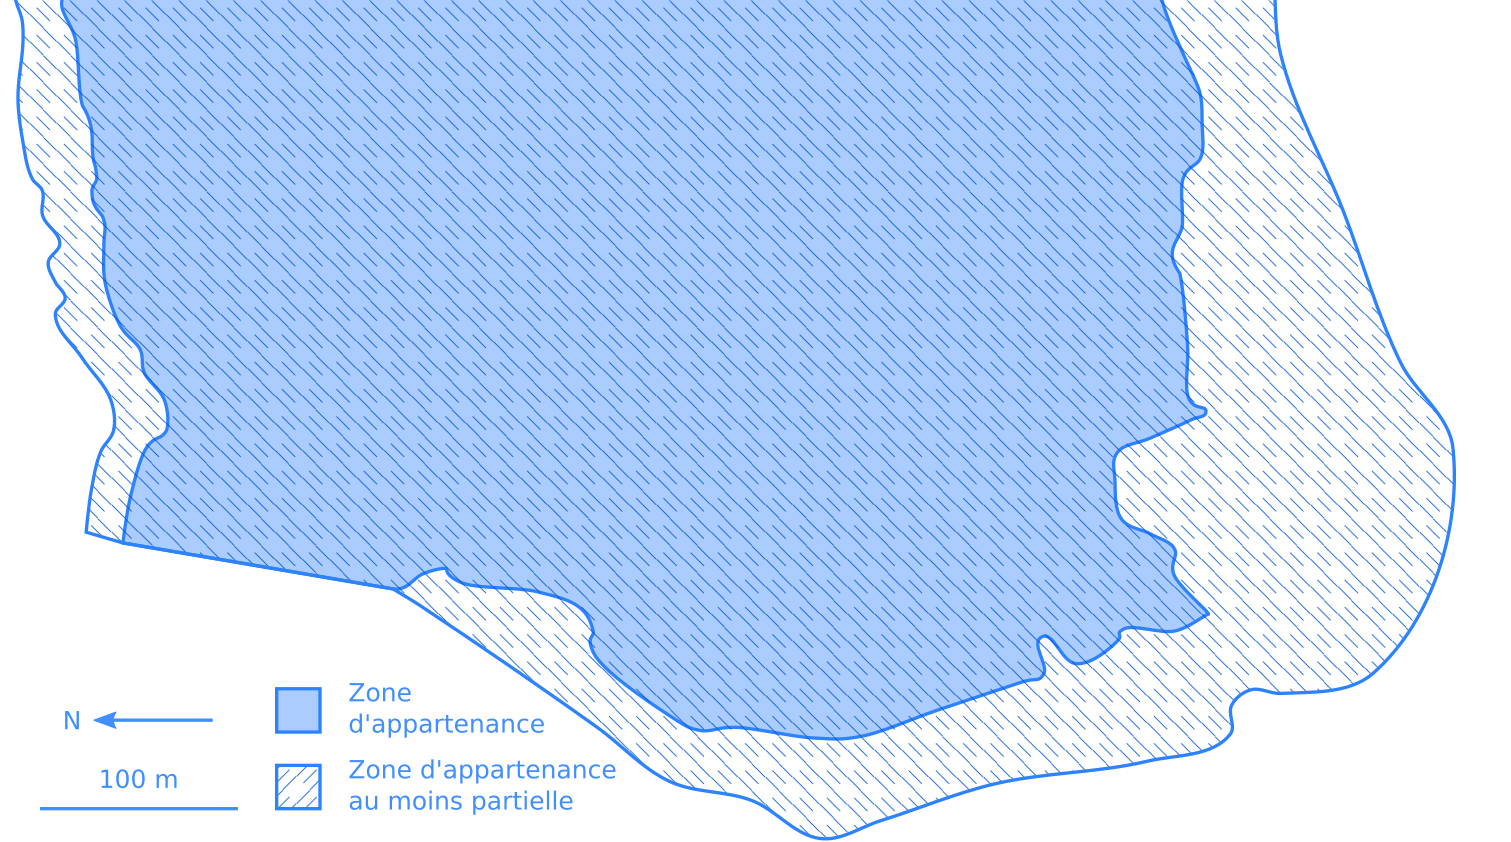
\includegraphics{../figures/fig7.png}
  \caption{Illustration de la modélisation du lac du Chambon avec un
    modèle exact tel que proposé par \textcite{Bejaoui2009}. Comme
    pour tous les modèles “exacts” la zone d’appartenance totale est
    incluse dans la zone d’appartenance au moins partielle. Extrait de
    \textcite{Bunel2020}.}
  \label{fig:champ_exact}
\end{figure}

\paragraph{Modèles et implémentation flous}

Définir un objet spatial imprécis à l’aide de la théorie des
sous-ensembles flous nécessite au préalable d’en élaborer un modèle de
représentation. C’est un travail qui, à notre connaissance, n’a été
entrepris que par \textcite{Schneider1999,Schneider2001} qui a
formalisé une version floue du modèle \emph{simple features.}

Le modèle de \textcite{Schneider1999} définit trois types de
géométries floues : le \emph{fpoint,} la \emph{fline} et la
\emph{fregion,} équivalents flous des types \emph{point, line} et
\emph{region} du modèle \emph{simple features.} La proposition de
\textcite{Schneider1999} se base sur le paradigme des ensembles de
points. Les fpoints sont définis comme une union de \emph{points
  flous} \footnote{}, \ie un ensemble de positions disjointes, deux à
deux, auxquelles est associée une valeur, le degré d’appartenance de
la position au \emph{fpoint.} Ainsi, contrairement à un \emph{point,}
un \emph{fpoint} peut occuper plus d’une position
(\autoref{fig:mod_schneider}). Les \emph{lignes floues} (à ne pas
confondre avec les \emph{flines}), sont également définies comme un
ensemble de \emph{points flous.} Cependant, contrairement au
\emph{fpoint,} la construction de cet ensemble est contrainte et les
points flous appartenant à une \emph{ligne floue} doivent se trouver
sur une même coube continue. De plus, chaque \emph{point flou} doit
avoir un degré d’appartenance unique, strictement croissant (ou
décroissant) dans le sens de la coube. Les deux \emph{points flous}
situés aux extrémités d’une \emph{ligne floue} ont donc,
respectivement, le degré d’appartenance maximal et minimal à la
\emph{ligne floue.} Les \emph{blocs flous} sont définis comme l’union
d’un nombre fini de \emph{lignes floues,} ne pouvant êtres connectées
que par leurs extrémités\footnote{} et les \emph{flines} comme une
union de \emph{blocs flous} disjoints. Cette construction permet aux
\emph{flines} de représenter des objets linéaires complexes et
composés de plusieurs géométries distinctes qui ne seraient pas
représentables par le type \emph{line} du modèle \emph{simple
  features} (Figure 8). Enfin, les \emph{fregions} sont définies comme
étant un ensemble de \emph{points flous} ne comportant pas d’anomalies
géométriques (\eg superpositions, croisements). Comme pour les
\emph{fpoints} et les \emph{flines,} les \emph{fregions} peuvent
modéliser des géométries plus complexes que le type \emph{region} du
modèle \emph{simple features}, une \emph{fregion} pouvant être
composée de plusieurs polygones disjoints
(\autoref{fig:mod_schneider}). \textcite{Schneider2004} complétera ce
modèle en définissant un ensemble de prédicats permettant de modéliser
des relations topologiques entre géométries floues.

\begin{figure}
  \centering
  \begin{tabular}{rC{3.5cm}C{3.5cm}C{3.5cm}}
  \toprule
  & \emph{fpoint} & \emph{fline} & \emph{fregion} \\
  \midrule
  \addlinespace[.5cm]
  \textbf{Cas simple} &
\includegraphics{../figures/SchneiderP1.pdf} &
                                                                      
\includegraphics{../figures/SchneiderP2.pdf}&
\includegraphics{../figures/SchneiderP3.pdf}\\
  \addlinespace[.5cm]
  \textbf{Cas complexe} &
\includegraphics{../figures/SchneiderP4.pdf} & 
\includegraphics{../figures/SchneiderP5.pdf}&
\includegraphics{../figures/SchneiderP6.pdf}\\
  \bottomrule
\end{tabular}

  \caption{Les trois types géométriques flous proposés par
    \textcite{Schneider1999}. D’après \textcite{Schneider1999} et
    \textcite{Bunel2020}.}
  \label{fig:mod_schneider}
\end{figure}

Plusieurs implémentations de ce modèle ont été proposées, notamment
par \textcite{Kanjilal2010} ou par \textcite{Dilo2006,Dilo2007}. Mais,
d’autres travaux ont également proposé des modélisations floues
d’objets spatiaux imprécis, sans rattachement ou définition explicite
d’un modèle théorique. C’est notamment le cas de \bsc{Zoghalmi} ou
\bsc{de Runz} qui proposent une approche fondée sur les
\emph{alpha-cuts} \autocite{de Runz2008,de
  Runz2008,Zoghlami2013,Zoghlami2016} ou de \textcite{Carniel2016}.

\textcite{Kanjina2100}, proposent d’implémenter le type fregion défini
par \textcite{Schneider1999} à l’aide de \enquote{région\textins{s}
  plateau}, définies comme un ensemble non nul et fini de
polygones\footnote{} (ou multi-polygones) nets, représentant une plage
de valeurs de degré d’appartenance. Cette implémentation est semblable
à l’approche par alpha-cuts proposée par \textcite{de Runz2008} ou
\textcite{Zoghalmi2013,Zoghalmi2016}. Dans la théorie des
sous-ensembles flous, une alpha-cut est définie comme l’ensemble des
éléments d’un sous-ensemble flou ayant un degré d’appartenance
supérieur à un seuil fixé \footnote{}
\autocite{Bouchon-Meunier2007}. Si les éléments du sous-ensemble flou
sont des positions, une alpha-cut permet de définir une aire,
modélisable par un polygone. Ainsi, les implémentations proposées par
\textcite{Kanjinal2010}, \textcite{Zoghalmi2013,Zoghalmi2016} ou
\textcite{de Runz2008} ont pour point commun de représenter un
sous-ensemble flou en le discrétisant à l’aide de polygones. Mais ces
approches ont une différence majeure: les contraintes de construction
des polygones. L’approche de \textcite{Kanjinal2010} impose aux
polygones constitutif d’une région plateau d’être disjoints ou
adjacents deux à deux, une même position ne peut donc appartenir qu’à
un seul polygone, ce qui n’est pas pour les implémentations proposées
par \textcite{Zoghalmi2013,Zoghalmi2016} ou \textcite{de Runz2008}, où
une position appartient, par définition, à toutes les alpha-cuts
construites à partir d’un seuil inférieur à son degré
d’appartenance. Cette distinction n’est pas visible sur la figure 9,
les deux approches donnant, pour le même nombre de polygones, des
résultats visuellement équivalents. Cependant, les trois polygones
représentés sur la figure 9 ont une sémantique différente selon
l’implémentation choisie. Dans l’implémentation de Kanjinal et
al. (2010), les trois polygones sont disjoints. Le premier délimite le
noyau, le second l’aire ayant un degré d’appartenance compris entre 1
et 0,25 (exclus) et le dernier polygone délimitant l’aire dont le
degré d’appartenance est strictement supérieur à 0 et inférieur à
0,25. Avec l’implémentation par alpha-cuts, les polygones sont
superposés, et si le premier polygone délimite toujours le noyau, le
second délimite l’aire dont le degré d’appartenance est supérieur à
0,25 et le troisième l’aire dont le degré d’appartenace est non
nul3. Par conséquent, si l’on ne construit que les alpha-cuts du noyau
et du support, le résultat de l’implémentation proposée par
\textcite{Zoghalmi2013,Zoghalmi2016} ou \textcite{de Runz2008} est
identique à celui des modèles de \textcite{Cohn1996} ou de
\textcite{Clementini1996} présentés précédemment et qui superposent
également la zone d’appartenance à la zone d’appartenance partielle;
ce qui n’est pas le cas pour l’implémentation de
\textcite{Kanjinal2010}, car les polygones définissant une région
plateau y sont, par définition, disjoints.

\begin{figure}
  \centering
  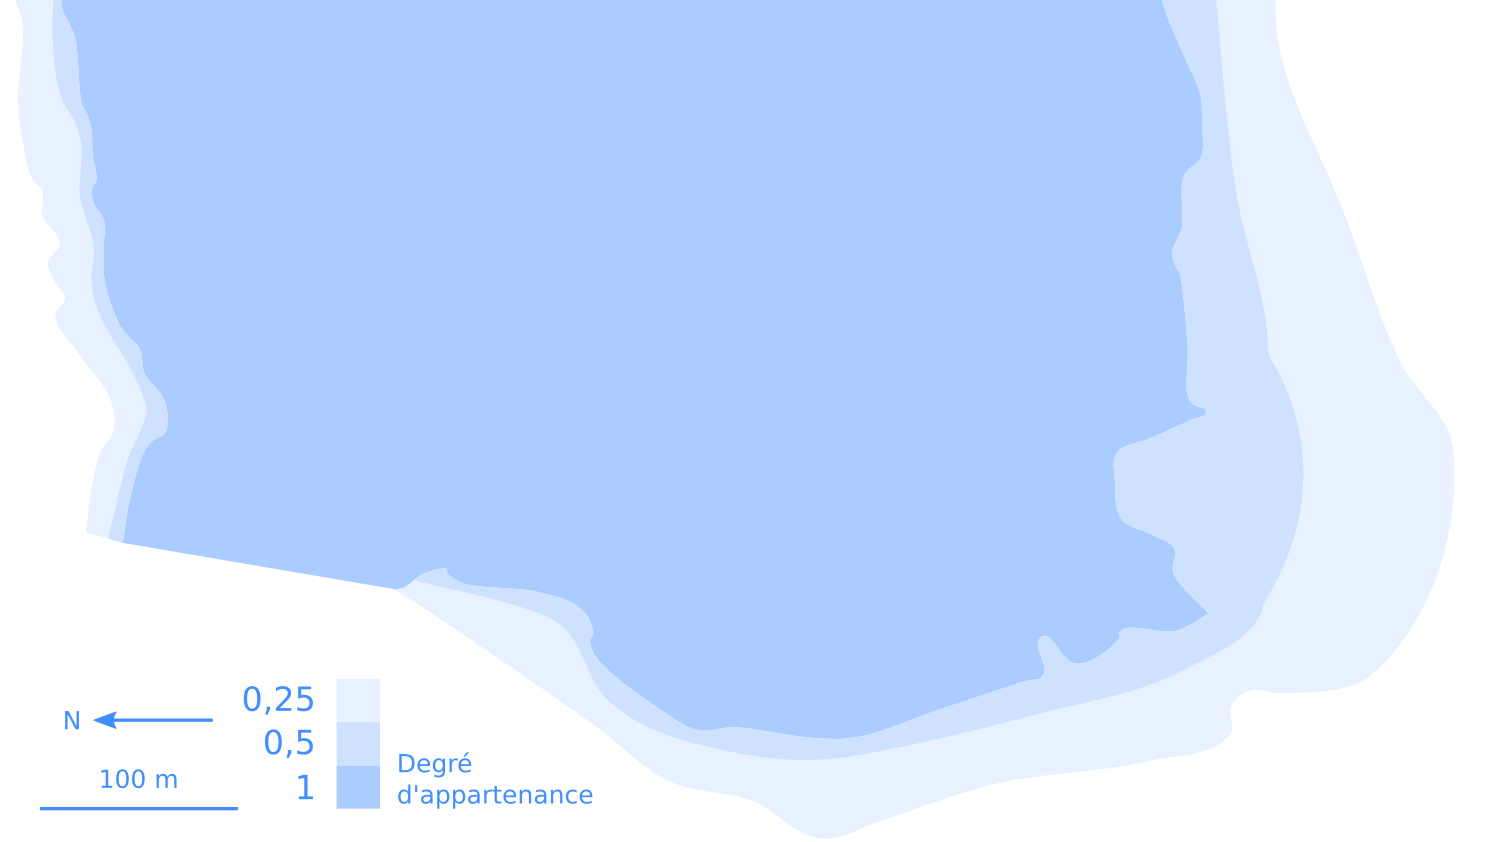
\includegraphics{../figures/fig9.png}
  \caption{Illustration de la modélisation du lac du Chambon avec un
    modèle flou discrétisé par un ensemble de polygones. Extrait de
    \textcite{Bunel2020}.}
  \label{fig:champ_polygones}
\end{figure}

Comme pour les implémentations précédentes, l’approche proposée par
\textcite{Dilo2007} ne s’applique qu’au cas des régions floues. Les
auteurs proposent d’implémenter ces dernières à l’aide de deux
linéaires, représentant les frontières du support et du noyau et d’un
maillage, servant de support à une interpolation. Les modèles
précédemment présentés imposent un échantillonnage des degrés
d’appartenance, dont la précision varie en fonction du nombre de
régions nettes \autocite{Kanjilal2010} ou d’alpha-cuts utilisées
\autocite{Zoghlami2016}. L’implémentation proposée par
\textcite{Zoghalmi2013,Zoghalmi2016} ou \textcite{de Runz2008} vise à
contourner ce problème en offrant la possibilité de calculer le degré
d’appartenance en tout point de la région floue par interpolation (de
manière similaire a la proposition de \textcite{Tossebro2002}. Ils
proposent pour cela de définir un maillage à l’aide d’une
triangulation de Delaunay contrainte aux frontières du noyau et du
support, cette dernière devant être post-traitée pour supprimer les
triangles créés dans les trous ou concavités. Le degré d’appartenance
au sous-ensemble flou des points appartenant aux frontières étant
connu, il est ainsi possible de calculer le degré d’appartenance en
tout point à l’aide d’une interpolation triangulaire (Figure 10). La
précision de l’estimation peut être améliorée par l’ajout de points
intermédiaires dont le degré d’appartenance à l’ensemble est connu, ce
qui peut être le cas lorsque, comme proposé par \textcite{Dilo2007},
la région floue est définie à partir d’un ensemble de points (les
frontières sont alors définies à l’aide d’enveloppes concaves). Le
principal problème de cette approche est qu’elle conduit à une
importante complexification des opérations inter-ensembles. Là où les
précédents modèles recouraient uniquement à des opérations
géométriques quelconques et à une sélection du plus grand (ou plus
petit, en fonction de l’opération concernée) degré d’appartenance, ce
modèle impose la reconstruction du maillage et son post-traitement, ce
qui peut rendre les opérations inter-ensembles (unions, intersections)
coûteuses.

\textcite{Schneider2003} a également proposé une implémentation de son
propre modèle. Contrairement aux implémentations précédemment citées,
celle-ci aborde tous les types formalisés dans le modèle théorique
(fpoint, fline et fregion). Ce travail est assez proche de ce qu’avait
proposé le même auteur avec sa proposition de modèle exact basé sur
l’approche Realm/Rose \textcite{Schneider1996}, puisque l’auteur
propose d’implémenter les types spatiaux flous à l’aide d’un ensemble
fini de points répartis régulièrement. L’implémentation du type fpoint
ne présente pas de particularités, il s’agit d’un point appartenant à
l’ensemble des positions possibles et ayant un degré
d’appartenance. De la même manière, l’implémentation du type fline est
proche de la formalisation, la principale différence étant que les
points composant cette dernière doivent nécessairement appartenir à
l’ensemble des positions possibles. Pour le type fregion ce dernier
est composé d’un ensemble de cellules auxquelles est attribué un degré
d’appartenance à la région floue. Les règles présentées dans le modèle
théorique s’appliquent toujours, ainsi les régions avec des anomalies
géométriques ne peuvent pas être modélisées. On peut noter que cette
implémentation des fregions est assez semblable à celle qui sera
proposée plus tardivement par \textcite{Kanjinal2010}, avec une région
floue modélisée comme un ensemble de polygones nets.

\begin{figure}
  \centering
  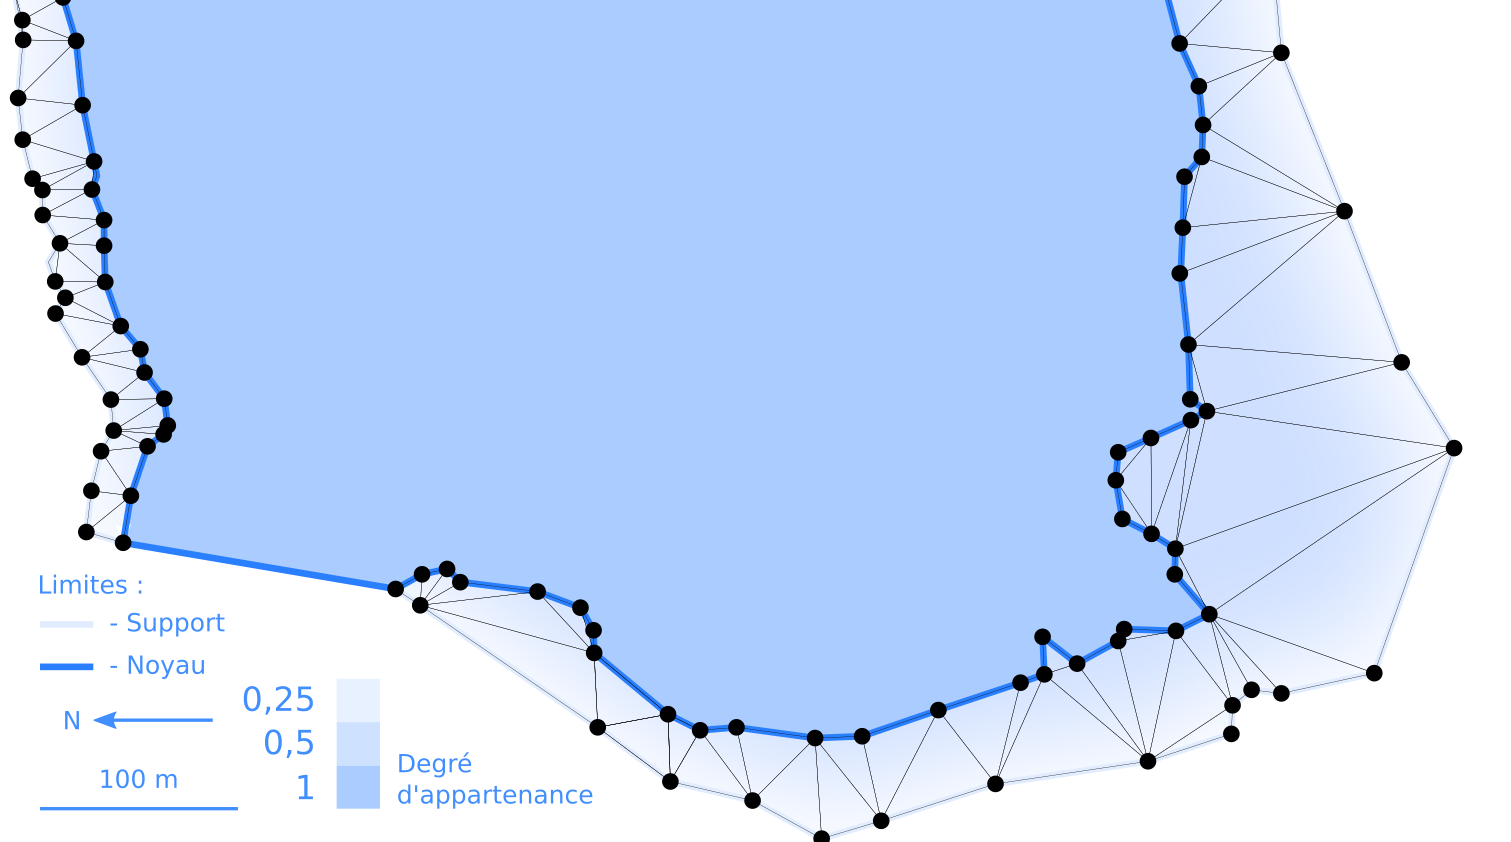
\includegraphics{../figures/fig10.png}
  \caption{Illustration de la modélisation du lac du Chambon avec un
    modèle flou tel qu’implémenté par \textcite{Dilo2007}. Extrait de
    \textcite{Bunel2020}.}
  \label{fig:champ_dilo}
\end{figure}

Pour finir, on peut également citer l’implémentation proposée par
\textcite{Carniel2016}. Ces derniers ne proposent qu’une
implémentation des lignes et des points flous, délaissant le cas des
régions floues. Cinq types sont définis et implémentés dans PostGIS
par les auteurs. Le premier d’entre eux est le type générique
FuzzyGeometry, qui se spécialise en FuzzyPoint, FuzzyLine et leurs
équivalents complexes, FuzzyMultiPoint et FuzzyMultiLine. On notera
que cette organisation reprend celle du modèle simple feature. Cette
ressemblance ne se limite pas à cet élément, puisque les types
complexes sont également définis comme des ensembles de types
simples. Les différences avec le modèle simple feature apparaissent
lors de la définition du type FuzzyPoint. Ce dernier est défini comme
un triplet composé de deux coordonnées x, y et d’un degré
d’appartenance. Par extension, le type FuzzyLine est défini comme un
ensemble de FuzzyPoint, ainsi le degré d’appartenance d’une FuzzyLine
est défini par les points qui la composent.

\subsubsection{Modèles basés sur une construction en extension}

Notre présentation des modèles basés sur une construction en extension
est organisée selon une classification \emph{ad hoc}, basée sur la
nature des objets sélectionnés (Partie 4.3.1) et distinguant les
modèles basés sur une construction en extension du premier ordre
(Partie 1.1.1) de ceux basés sur une construction en extension d’ordre
supérieur (Partie 1.1.13).

\paragraph{Critères de classement}

Comme nous l’expliquions précédemment, toute définition d’un objet
spatial par la sélection d’un ou plusieurs objets géographiques est
une construction en extension. On peut distinguer ces modèles selon la
nature des objets spatiaux sélectionnés.

Une première possibilité consiste à définir un objet spatial par la
sélection des positions qu’il occupe. La délimitation d’une zone à
partir d’un ensemble de pixels est un exemple concret de ce type
d’approche, notamment proposée par \textcite{Zhan1997}. Cet exemple ne
doit cependant pas laisser croire que la catégorisation proposée ici
est fondée sur la nature de l’implémentation, mais bien sur la
sélection de positions dont l’infinité ne peut qu’être approximée par
des modèles champs, quelle que soit la nature de leur
implémentation. Toutefois, l’ensemble des travaux que nous
présenterons s’appuie sur une approche raster.

À l’inverse, on peut imaginer construire des objets spatiaux à partir
d’une sélection d’objets, d’ « agrégats » \autocite{Charrre1995} de
positions. Cette approche définit des objets spatiaux de manière
semblable aux\emph{ Elements-Clustering Objects} de \textcite{Liu2019}
(Partie 2.2). Dans ce cas, le sous-ensemble spatialisé peut être
défini à partir d’un groupe d’éléments ne couvrant pas l’intégralité
de l’espace (\eg sélection à partir d’un réseau routier). Nous
qualifions ce second type de sélection d’ordre supérieur, car elle
s’opère sur des objets complexes, eux-mêmes composés de positions, et
non directement de positions comme c’est le cas pour une sélection
directe de positions, que nous qualifions de sélection de premier
ordre.

\paragraph{Construction en extension du premier ordre}

On peut présenter la définition en extension du premier ordre d’un
sous-ensemble flou spatialisé à l’aide de l’exercice de définition
d’une limite pour le lac du Chambon. La Figure 11 se distingue des
exemples précédents par son découpage en pixels (dont la taille a
volontairement été exagéré). Chacun se voit attribuer un degré
d’appartenance, défini indépendamment. La tâche principale consiste
donc à définir une méthode permettant de calculer le degré
d’appartenance pour chaque pixel. Pour cet exemple, nous avons adopté
une approche simple : le degré d’appartenance décroit avec la distance
au rivage. Le degré d’appartenance est donc de 1 pour les pixels
situés à l’intérieur du lac, puis il décroit en fonction de la
distance du centroïde du pixel au point du rivage le plus proche. Ces
règles peuvent être raffinées autant que nécessaire.

Les travaux de \textcite{Vanegass2011,Takemura2012}, par exemple,
s’intéressent à la modélisation de relations spatiales, respectivement
« entouré de » et « le long de ». L’objectif est de délimiter la zone
validant la relation spatiale considérée, c’est-à-dire de construire
un « paysage flou » selon la terminologie proposée par
\textcite{Bloch1996}. Ce type de modélisation est nécessairement
impacté par l’imprécision du langage naturel. Une description de
position est nécessairement imprécise, une même relation spatiale
pouvant prendre un sens différent en fonction de l’objet de référence,
du locuteur, etc. \autocite{Vandeloise1986,Borillo1998,Bateman2010},
écueil justifiant le recours à la théorie des sous-ensembles
flous. Ces deux travaux sont fondés sur une méthodologie
similaire. Ils définissent tous deux un ensemble de métriques et de
fonctions permettant de calculer, pour chaque pixel d’un raster, un
degré d’appartenance quantifiant la validité de la relation spatiale
modélisée pour la position considérée.

\begin{figure}
  \centering
  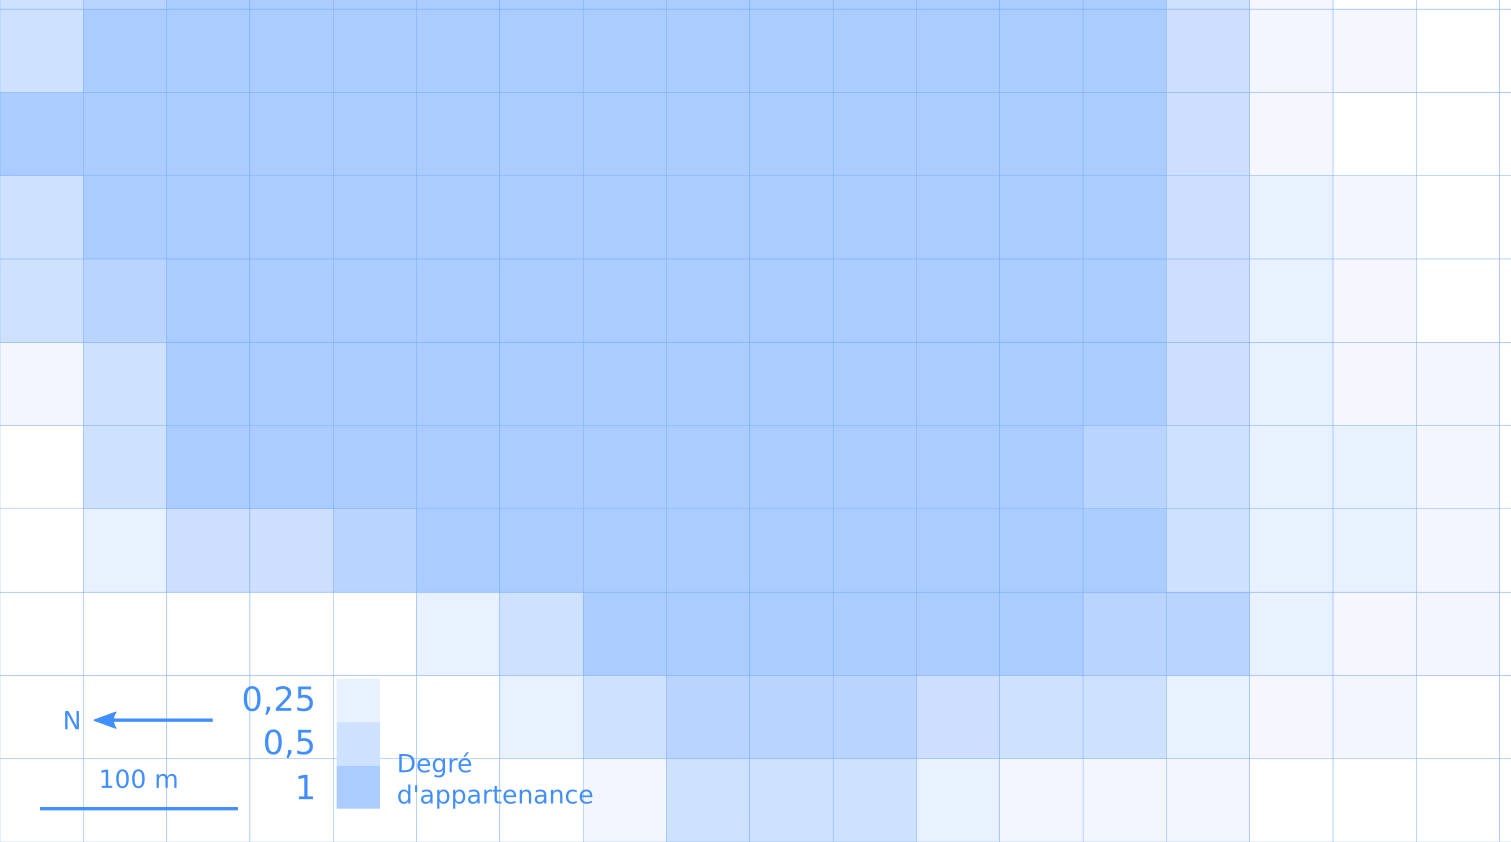
\includegraphics{../figures/fig11.png}
  \caption{Illustration de la modélisation du lac du Chambon par un
    modèle flou et une implémentation raster (\ie construction en
    extension de premier ordre). Extrait de \textcite{Bunel2020}.}
  \label{fig:champ_raster}
\end{figure}

Si ces travaux proposent avant tout une réflexion théorique, d’autres
auteurs utilisent cette même approche pour répondre à des
problématiques plus appliquées. C’est notamment le cas
d’\textcite{Arabacioglu2010} qui propose une application de la théorie
des sous-ensembles flous à l’architecture, ou
\textcite{Kurtener2000,Makropoulos2003,Girot2007} qui se sont penchés
sur des questions de prise de décision appliquées à la gestion du
territoire. Comme précédemment, ces travaux utilisent un raster et
calculent pour chaque pixel un degré d’appartenance à une zone, dont
la sémantique varie en fonction de la problématique. Cependant, le
calcul du degré d’appartenance dans les travaux de
\textcite{Griot2007,Makropoulos2003,Arabacioglu2010} est réalisé à
l’aide d’un système d’inférence flou et non directement comme dans les
travaux de \textcite{Vanegass2011,Takemura2012}. Les systèmes
d’inférence flous, pendant flou des systèmes experts, permettent
également de calculer un degré d’appartenance pour chaque individu
(quelle que soit sa nature), mais à partir de règles logiques
formulées en langage naturel.  Leur utilisation permet donc de prendre
en compte l’imprécision, ici liée à l’expression orale
\autocite{Makropoulos2003,Griot2007}, ou à la quantification de
ressentis \autocite{Arabacioglu2010}, mais également de formaliser des
connaissances expertes.

La définition en extension du premier ordre d’un sous-ensemble
spatialisé est courante dans la littérature et les publications
présentées ici, l’appliquent à des thématiques diverses, comme
l’interprétation d’images aériennes \autocite{Brandtberg2002,
  Fonte2005}, la gestion du territoire
\autocite{Griot2007,Makropoulos2003}, la qualification de ressentis
\autocite{Arabacioglu2010}, ou la modélisation de relations spatiales
floues \textcite{Vanegass2011,Takemura2012}.

\paragraph{Construction en extension d'ordre supérieur}

La construction en extension d’ordre supérieur d’un sous-ensemble flou
spatialisé est probablement l’approche qui nécessite le plus de
s’appuyer sur un exemple concret (Figure 12). Comme nous l’expliquions
précédemment, cette approche nécessite d’attribuer des degrés
d’appartenance à des objets, des agrégats de position. Elle se
distingue donc de la construction en extension du premier ordre, qui
nécessite d’attribuer un degré d’appartenance à des positions (cas
théorique) ou à un pavage régulier, une discrétisation de l’ensemble
des positions (cas pratique, cf. Figure 11). La Figure 12 représente à
la fois l’occupation du sol de la zone traitée et le degré
d’appartenance1 de l’objet à la zone modélisée. Ainsi, on considère
que le polygone du lac appartient totalement au sous-ensemble flou
“lac”, que les berges y appartiennent moyennement et qu’une partie des
forêts y appartient faiblement. Quant aux autres éléments, on
considère qu’ils n’appartiennent pas à la zone modélisée.

\begin{figure}
  \centering
  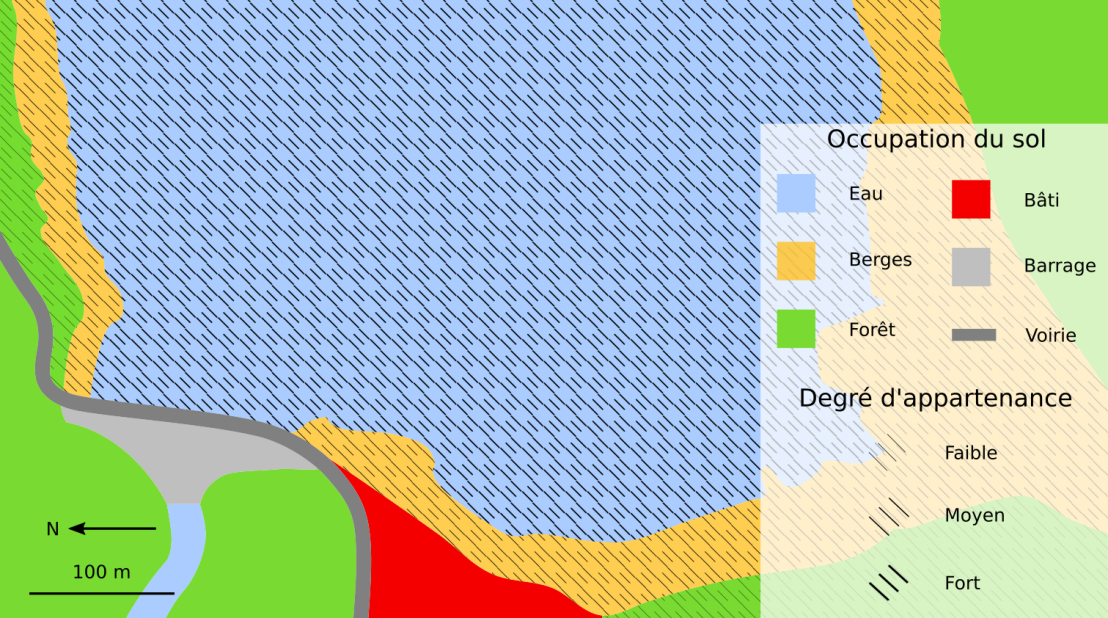
\includegraphics{../figures/fig12.png}
  \caption{Illustration de la définition du lac du Chambon par
    sélection floue d’objets géographiques (\ie construction en
    extension d’ordre supérieur). Extrait de \textcite{Bunel2020}.}
  \label{fig:champ_raster_sel}
\end{figure}

Ce processus de construction, pendant spatial de la réflexion sur les
requêtes floues \textcite{Wang1994,Moreau2018}, est utilisé par
\textcite{Duraciova2017} qui illustrent leur méthodologie par la
sélection floue « [des] grands parkings proches du stade et ayant été
rénovés il y a environ deux ans ». Leur démarche est fortement
similaire à celle de l’exemple précédent (Figure 12). Les autrices
définissent des règles permettant de quantifier l’appartenance des
objets spatiaux candidats à l’ensemble flou correspondant à la
description. Là où nous n’utilisions qu’un seul critère, la proximité,
ce nouvel exemple nécessite de prendre en compte la proximité mais
aussi la date de la dernière rénovation. Chacun de ces critères permet
de construire un sous-ensemble flou spatialisé (celui des parkings
proches du stade et celui des parking rénovés il y a environ deux ans)
et l’intersection de ces deux ensembles, réalisée à l’aide des
opérateurs flous présentés précédemment (Partie 3) permet de
construire le sous-ensemble flou désiré. Un processus similaire est
utilisé par \textcite{Bard2003} dans le cadre de l’évaluation de la
généralisation cartographique. Les objets spatiaux sont ici classés
dans des sous-ensembles flous figurant une description qualitative de
la qualité de la généralisation. \textcite{Cross2000} utilisent quant
à eux une approche similaire pour ajouter la prise en compte de
l’imprécision aux modèles objets des systèmes d’information
géographiques. Dans tous les cas, le sous-ensemble flou construit est
spatialisé, mais cette spatialisation est exogène, puisque dépendante
de la géométrie des objets spatiaux sélectionnés.

% Conclusion de cybergéo

Dans cet état de l’art, nous avons souhaité présenter les différents
concepts permettant de décrire les objets géographiques dont la
délimitation précise est impossible. Les différentes théories et
implémentations recensées offrent de nombreuses possibilités pour
modéliser l’imprécision spatiale. Nous nous sommes particulièrement
penché sur les différentes implémentations que nous avons catégorisées
selon leur méthode de construction. Ainsi, nous distinguons les
implémentations basées sur une construction en intension et les
implémentations basées sur une construction en extension.

La modélisation de l’imprécision spatiale est donc un champ de
recherche riche, qui offre au géographe de nombreux outils théoriques
permettant de travailler efficacement avec les nombreux objets
spatiaux aux frontières imprécises auxquels nous sommes régulièrement
confrontés. Bien que la considération de l’imprécision des objets
spatiaux soit assez ancienne, la formalisation de modèles et encore
plus leur implémentation, est un champ de recherche encore actif comme
le montre, par exemple, la récente réflexion autour de l’expression de
l’imprécision spatiale au sein du format GML \autocite{Wei2017}.


%%% Local Variables:
%%% mode: latex
%%% TeX-master: "../../../../main"
%%% End:
